\chapter{Dynamická měření}
Dynamická měření přísunů radonu jsem provedl u tří objektů, viz tab.~\ref{tab:dynMer_prehled}.
\begin{table}[ht]
	\centering
	\caption{Objekty, v nichž jsem provedl dynamická měření. $T$ značí dobu měření ve dnech (zaokrouhleno na celé dny včetně počátečního a posledního dne).}
	\label{tab:dynMer_prehled}
	\begin{tabular}{llll}
		\toprule
		Objekt & Rozsah měření & $T$ [dny] & Typ objektu\\
		\midrule
		Skála 75, okr. Havlíčkův Brod & 23. 5. -- 5. 6. 2019 & 14 & chata\\
		Hálková 980, Humpolec & 5. 6. -- 20. 6. 2019 & 16 & byt\\
		Anglická 574, Dobřichovice & 9. 7. -- 30. 7. 2019 & 22 & rodinný dům\\
		\bottomrule
	\end{tabular}
\end{table}

Vývoj OAR v čase v jednotlivých zónách byl měřen primárně \emph{TERA sondami}~\cite{tera} a sekundárně měřiči radonu \emph{CANARY}~\cite{canary}. CANARY měřáky byly použity jako záložní systém, tj. pokud by v některé zóně  TERA sonda selhala, pak by se OAR v této zóně brala z příslušného CANARY měřáku. %Zevrubné informace o těchto detektorech lze dohledat v kapitole~\ref{navesti:radon}.

Dále bylo potřeba měřit vývoj teploty, což je znalost nutná při vyhodnocování množství nasorbovaných indikačních plynů v TD detektorech. K tomuto účelu byly použity dataloggery teploty a vlhkosti \emph{testo 174H} \cite{testo}.

Před samotnými měřeními přísunů radonu v objektech bylo nejprve nutno provést srovnávací měření TERA sond, jelikož každá sonda má různou odezvu při stejné OAR. O tomto pojednává podkapitola~\ref{navesti:dynMer_TERA}. Další podkapitoly obsahují dynamická měření přísunů radonu v uvedených objektech. 
\section{TERA sondy}\label{navesti:dynMer_TERA}
Pro dynamická měření přísunů radonu mi byly poskytnuty čtyři TERA sondy s označením 8, 10, 88 a 112. Pro srovnání jejich odezev s reálnou hodnotou OAR byly vloženy do sudu (nádoba válcovitého tvaru) spolu s referenčním monitorem radonu \emph{AlphaGuard} \cite{alphaguard}. Hodnota OAR z AlphaGuardu byla brána jako reálná hodnota OAR. V obr.~\ref{fig:dynMer_sondySrovnani} jsou zobrazeny naměřené vývoje OAR v čase ze zkoumaných sond a z Alphaguardu, v tab.~\ref{tab:dynMer_sondy} jsou k vidění nejdůležitější statistiky naměřených dat z každého monitoru.

\begin{figure}[H]
	\centering
	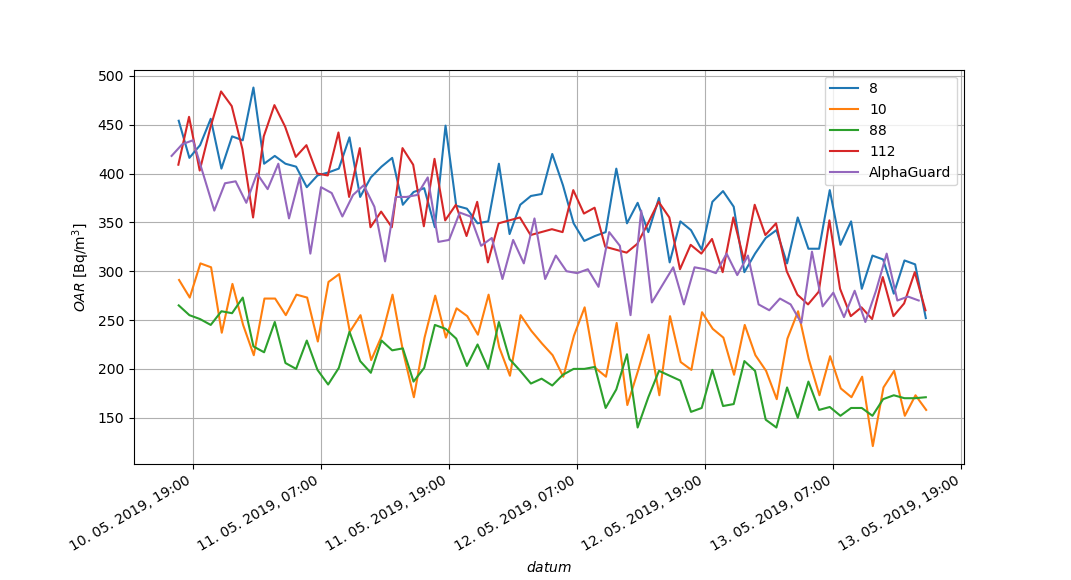
\includegraphics[width=1\linewidth]{images/sondy_srovnani}
	\caption{Vývoj OAR naměřený zkoumanými sondami a referenčním AlphaGuardem.}
	\label{fig:dynMer_sondySrovnani}
\end{figure}
\begin{table}[ht]
	\centering
	\caption{Statistiky vývojů OAR naměřených TERA sondami a AlphaGuardem v \si{Bq/m^3}.}
	\label{tab:dynMer_sondy}
	\begin{tabular}{lrrrrrrrr}
		\toprule
		ID sondy &  count &  mean &  std &  min &  25\% &  50\% &  75\% &  max \\
		\midrule
		8          &     71 &   369 &   47 &  252 &  337 &  368 &  405 &  488 \\
		10         &     71 &   228 &   41 &  121 &  198 &  232 &  256 &  308 \\
		88         &     71 &   198 &   33 &  140 &  170 &  198 &  220 &  273 \\
		112        &     71 &   354 &   58 &  251 &  318 &  349 &  399 &  484 \\
		\midrule
		AlphaGuard &     71 &   328 &   50 &  247 &  285 &  318 &  373 &  434 \\
		\bottomrule
	\end{tabular}
\end{table}

Pro opravu odezev byla zavedena pro každou sondu tzv. bulharská konstanta, která je definována následovně:
\begin{equation}
	B=\frac{OAR_A}{OAR_T}\,,
\end{equation}
kde $OAR_A$ je hodnota z AlphaGuardu a $OAR_T$ je hodnota z příslušné TERA sondy. Pro získání věrohodné hodnoty koncentrace radonu z naměřené hodnoty danou sondou pak stačí tuto naměřenou hodnotu přenásobit $B$ náležející této sondě.

Za $OAR_A$, resp. $OAR_T$ byly brány průměry naměřených OAR AlphaGuardem a danou Tera sondou. Relativní nejistoty bulharských konstant byly odhadnuty na 10~\%. Určené bulharské konstanty všech sond jsou k nahlédnutí na obr.~\ref{fig:dynMer_sondyB} a v tab.~\ref{tab:dynMer_sondyB}. %Nejistoty bulharských konstant určeny nebyly vzhledem k tomu, že se jedná o "veličinu", která se může při různých vnějších podmínkách měnit. Hlavním ovlivňujícím faktorem je velikost aerosolů v měřeném prostředí. Tato nespolehlivost TERA sond v poskytování věrohodných dat je dalším důvodem, proč byly použity měřáky radonu CANARY. Takto můžeme srovnávat data z více zdrojů.
\begin{figure}[H]
	\centering
	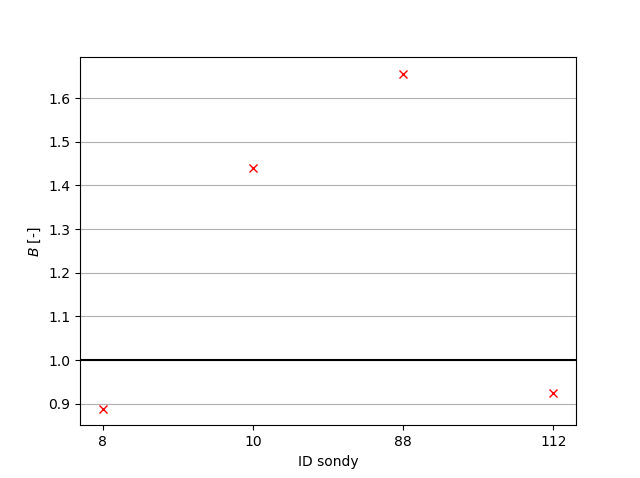
\includegraphics[width=0.7\linewidth]{images/sondy_B}
	\caption{Bulharské konstanty proměřených TERA sond. Černou čárou je vyznačen ideální případ, kdy se odezva sondy rovná skutečné OAR (resp. OAR naměřené AlphaGuardem).}
	\label{fig:dynMer_sondyB}
\end{figure}
\begin{table}[ht]
	\centering
	\caption{Bulharské konstanty TERA sond odvozené od referenčního AlphaGuardu. Skutečná hodnota $OAR$ se vypočte ze vztahu $OAR=B\cdot OAR_T$, kde $OAR_T$ je naměřená obj. aktivita radonu danou TERA sondou. Nejistota bulharských konstant byla odhadnuta na 10~\%.}
	\label{tab:dynMer_sondyB}
	\begin{tabular}{lr}
		\toprule
		ID sondy &     $B$ \\
		\midrule
		8   & 0,889+/-0,089\\
		10  & 1,440+/-0,140\\
		88  & 1,655+/-0,166\\
		112 & 0,925+/-0,093\\
		\bottomrule
	\end{tabular}
\end{table}
\section{Objekt Skála 75, okr. Havlíčkův Brod}
\subsection{Použitá měřidla}
\begin{itemize}
    \setlength\itemsep{0em}
	\item 14 vyvíječů (2x TMH, 2x TCE, 3x MDC, 3x MCH, 2x PCE, 2x PCH)
	\item 12 TD detektorů
	\item 4 CANARY monitory
	\item 4 TERA sondy
	\item 3 TESTO měřiče teploty a vlhkosti
	\item 2 zdroje radonu
\end{itemize}
\begin{table}[H]
    \centering
    \caption{Objemy podlaží objektu, teploty naměřené v každém podlaží dataloggery testo 174H, odhadnuté atmosférické tlaky v každém podlaží a přiřazení číslování kompartmentů jednotlivým podlažím.}
    \label{tab:skala75_objemy}
    \begin{tabular}{lll}
\toprule
podlazi & $OAR$ [\si{Bq/m^3}] & $V$ [\si{m^3}] \\
\midrule
0 &           1094+/-55 &         40+/-8 \\
1 &            562+/-20 &        84+/-10 \\
2 &              51+/-2 &        97+/-15 \\
\bottomrule
\end{tabular}

\end{table}
\begin{table}[H]
    \centering
    \caption{Přehled použitých indikačních plynů. $M$ je molekulová hmotnost příslušného plynu, $U$ je jeho odběrová rychlost. Dále je uvedeno, v jakém podlaží byly vyvíječe plynů umístěny s jejich celkovými odpary za celou dobu měření. Význam označení podlaží je vysvětlen v tab. \ref{tab:rovMer_podlazi}.}
    \label{tab:skala75_indikacniPlyny}
    \begin{tabular}{lrrrr}
\toprule
ozn. & podlaží& odpar [mg] &    $M$ [g/mol] &    $U$ $\left[\si{\frac{ng}{ppm\cdot min}}\right]$\\
\midrule
TMH & 0 &192,50 &  450,0 &  8,000 \\
TCE & 0 &193,55 &  130,4 &  1,000 \\
MCH & 1 &472,27 &  350,0 &  8,000 \\
MDC & 1 &497,27 &  400,0 &  8,000 \\
PCH & 2 &230,88 &  450,0 &  8,000 \\
PCE & 2 & 96,54 &  165,8 &  1,385 \\
\bottomrule
\end{tabular}

\end{table}
\begin{table}[H]
    \centering
    \caption{Odezvy TD detektorů $R$ na všechny použité indikační plyny ve všech zónách.}
    \label{tab:skala75_odezvyTD}
    \begin{tabular}{lrr}
\toprule
plyn & zóna & $R$ [\si{ng}]               \\
\midrule
MCH & 1 & $  36,0\pm2,3$\\
    & 2 & $395,8\pm16,6$\\
    & 3 & $  50,8\pm2,3$\\
MDC & 1 & $  34,5\pm1,2$\\
    & 2 & $ 304,9\pm7,1$\\
    & 3 & $  47,2\pm1,2$\\
TMH & 1 & $145,3\pm26,0$\\
    & 2 & $  37,5\pm3,9$\\
    & 3 & $  20,2\pm2,4$\\
PCH & 1 & $  20,7\pm2,4$\\
    & 2 & $  26,9\pm0,7$\\
    & 3 & $ 182,2\pm4,6$\\
TCE & 1 & $191,8\pm14,5$\\
    & 2 & $  32,2\pm1,4$\\
    & 3 & $  25,0\pm1,2$\\
PCE & 1 & $     0,0\pm0,0$\\
    & 2 & $   2,6\pm0,1$\\
    & 3 & $ 136,9\pm4,1$\\
\bottomrule
\end{tabular}

\end{table}

\subsection{Naměřené OAR}
\begin{figure}[H]
    \centering
    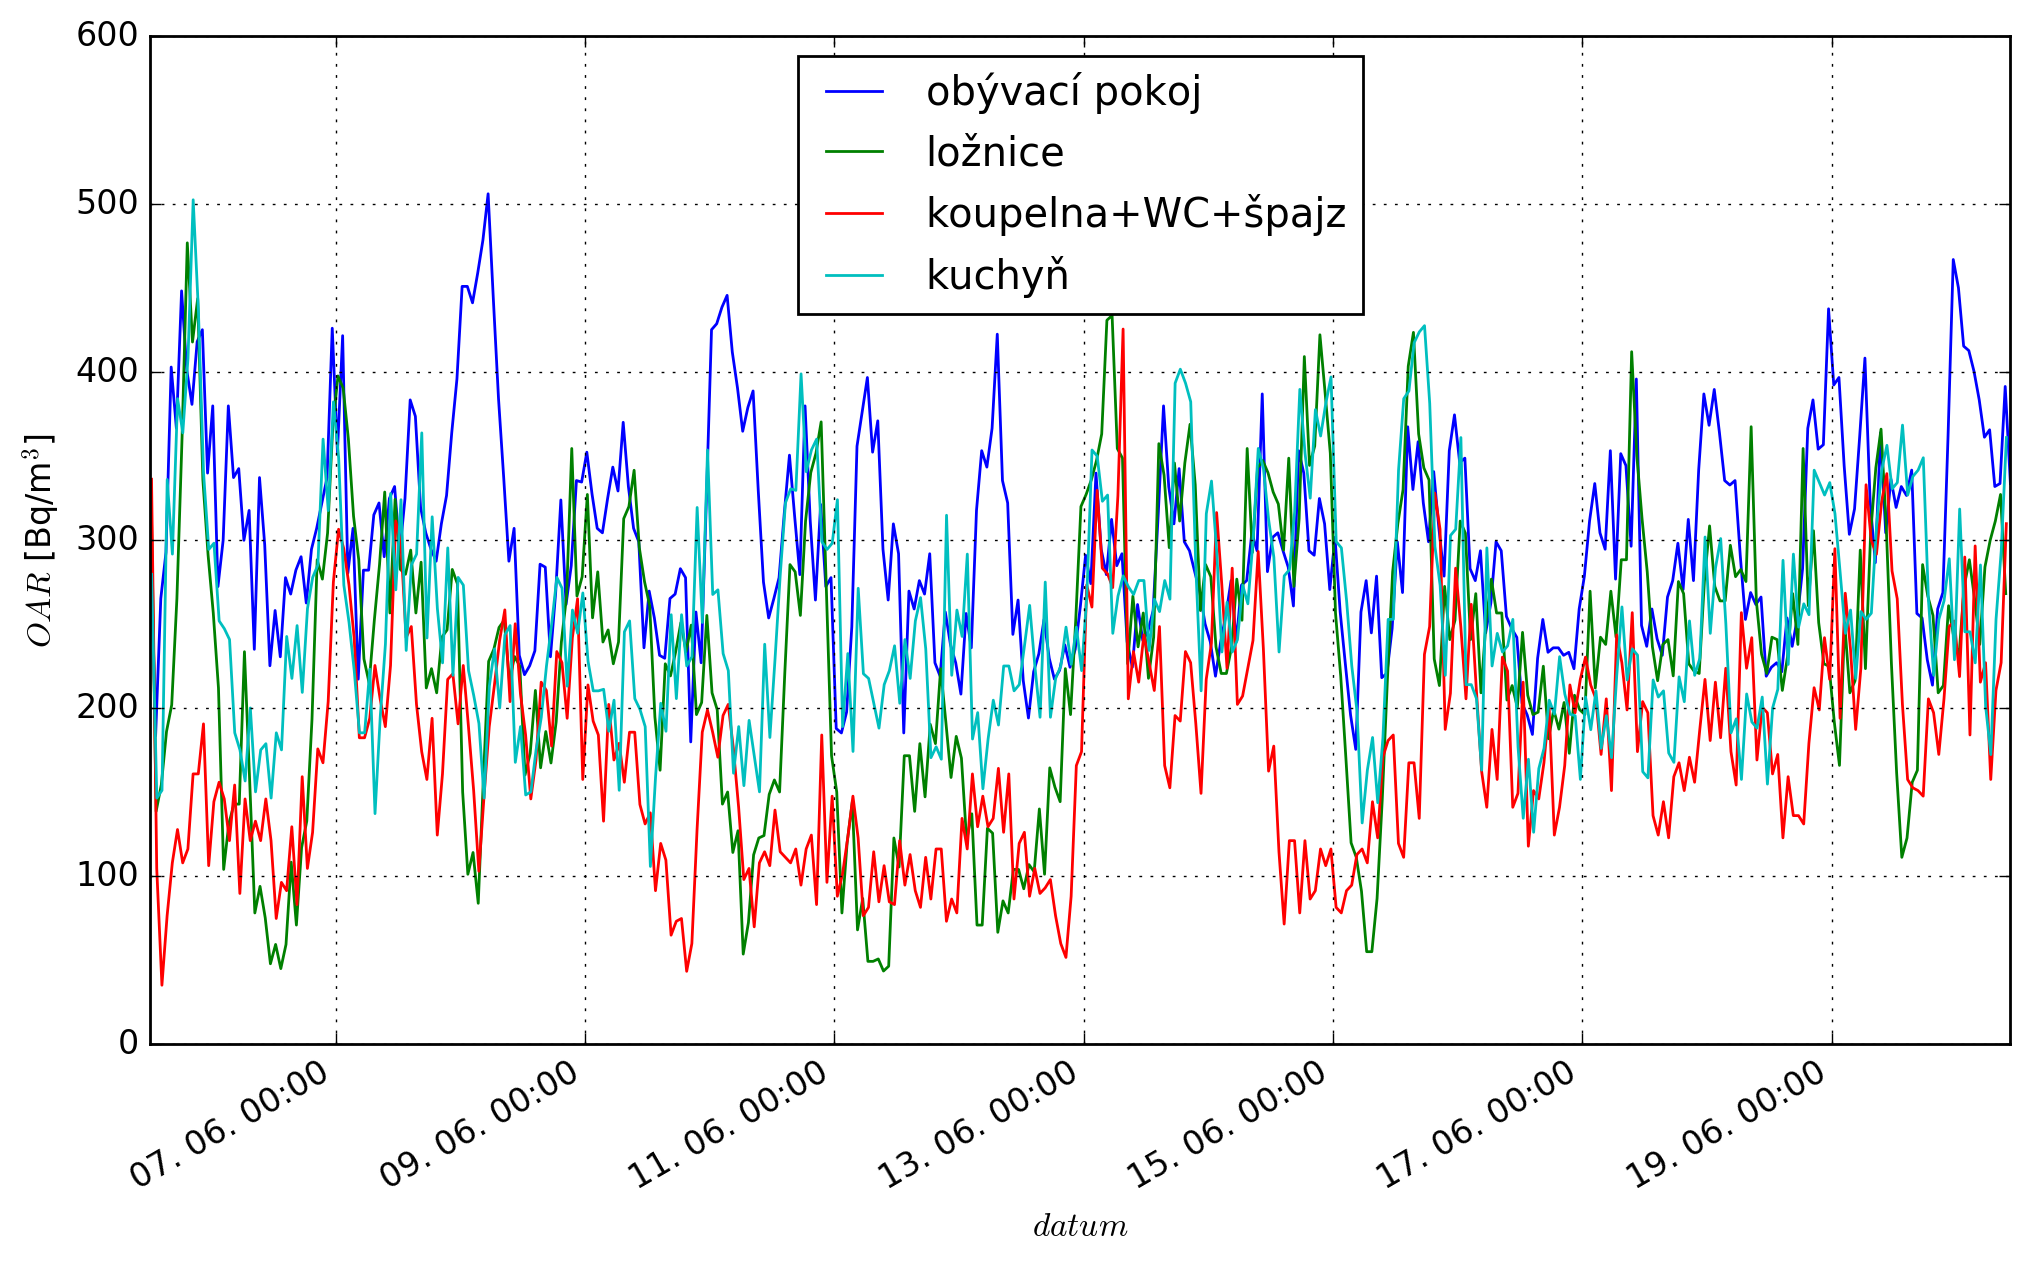
\includegraphics[width=1\textwidth]{skala75/OAR_dohromady.png}
    \caption{Hodnoty OAR naměřené TERA sondami po aplikování bulharských konstant (tab.~\ref{tab:dynMer_sondyB}). Pro další vyhodnocování byly OAR naměřené v přízemí v kuchyni a v ložnici zprůměrovány.}
    \label{fig:skala75_OARdohromady}
\end{figure}
\subsection{Objemové průtoky vzduchu}

\begin{table}[H]
    \centering
    \caption{Objemové průtoky vzduchu v \si{m^3/hod} pro všechny kombinace aplikovaných indikačních plynů. $n$ je výměna vzduchu vypočtená ze vztahu~\eqref{eq:prutoky_n}, $[n]=\si{1/hod}$.}
    \label{tab:skala75Prutoky_celkove}
%\begin{tabular}{l>{\raggedleft\arraybackslash}p{2.5cm}>{\raggedleft\arraybackslash}p{2.5cm}>{\raggedleft\arraybackslash}p{2.5cm}>{\raggedleft\arraybackslash}p{2.5cm}}
%\toprule
%{} & (TMH, MDC, PCE) & (TMH, MDC, PCH) & (TMH, MCH, PCE) & (TMH, MCH, PCH)\\ 
%\midrule
%$k_{12}$ & 4.139$\pm$1.044 & 3.771$\pm$0.994 & 3.445$\pm$0.874 & 3.128$\pm$0.830 \\          
%$k_{13}$ & 0.478$\pm$0.133 & 1.892$\pm$0.533 & 0.495$\pm$0.136 & 1.956$\pm$0.541 \\          
%$k_{21}$ & 0.656$\pm$0.152 & 0.574$\pm$0.137 & 0.525$\pm$0.126 & 0.455$\pm$0.114 \\          
%$k_{23}$ & 0.202$\pm$0.030 & 0.800$\pm$0.119 & 0.167$\pm$0.026 & 0.660$\pm$0.104 \\          
%$k_{31}$ &-0.019$\pm$0.005 & 0.854$\pm$0.233 &-0.015$\pm$0.004 & 0.881$\pm$0.237 \\          
%$k_{32}$ & 0.231$\pm$0.034 & 1.882$\pm$0.282 & 0.192$\pm$0.029 & 1.561$\pm$0.240 \\          
%$k_{1_E}$&12.492$\pm$2.813 &11.640$\pm$2.705 &13.100$\pm$2.886 &12.163$\pm$2.768 \\          
%$k_{2_E}$& 7.169$\pm$0.789 & 6.809$\pm$0.790 & 5.990$\pm$0.690 & 5.674$\pm$0.686 \\          
%$k_{3_E}$& 1.930$\pm$0.212 & 5.749$\pm$0.804 & 1.964$\pm$0.213 & 6.010$\pm$0.804 \\          
%$k_{1_I}$&16.471$\pm$3.007 &15.875$\pm$2.943 &16.530$\pm$3.022 &15.912$\pm$2.952 \\          
%$k_{2_I}$& 3.657$\pm$1.318 & 2.530$\pm$1.313 & 3.045$\pm$1.122 & 2.099$\pm$1.114 \\          
%$k_{3_I}$& 1.462$\pm$0.255 & 5.793$\pm$1.039 & 1.478$\pm$0.256 & 5.836$\pm$1.032 \\          
%\midrule
%$n$      & 0.091$\pm$0.014 & 0.102$\pm$0.015 & 0.089$\pm$0.014 & 0.101$\pm$0.015 \\
%\bottomrule
%\end{tabular}
%\vspace{0.5cm}

%\begin{tabular}{l>{\raggedleft\arraybackslash}p{2.5cm}>{\raggedleft\arraybackslash}p{2.5cm}>{\raggedleft\arraybackslash}p{2.5cm}>{\raggedleft\arraybackslash}p{2.5cm}}
    %\toprule
    %{} & (TCE, MDC, PCE) & (TCE, MDC, PCH) & (TCE, MCH, PCE) & (TCE, MCH, PCH) \\
    %\midrule
%$k_{12}$ & 3.330$\pm$0.551 & 2.965$\pm$0.519 & 2.774$\pm$0.468 & 2.462$\pm$0.438 \\
%$k_{13}$ & 0.462$\pm$0.081 & 1.828$\pm$0.322 & 0.476$\pm$0.082 & 1.879$\pm$0.326 \\
%$k_{21}$ & 0.215$\pm$0.034 & 0.188$\pm$0.032 & 0.172$\pm$0.030 & 0.149$\pm$0.028 \\
%$k_{23}$ & 0.203$\pm$0.029 & 0.802$\pm$0.118 & 0.168$\pm$0.026 & 0.662$\pm$0.104 \\
%$k_{31}$ &-0.006$\pm$0.001 & 0.279$\pm$0.060 &-0.005$\pm$0.001 & 0.288$\pm$0.061 \\
%$k_{32}$ & 0.230$\pm$0.034 & 1.922$\pm$0.283 & 0.191$\pm$0.029 & 1.595$\pm$0.241 \\
%$k_{1_E}$& 1.805$\pm$0.627 & 0.865$\pm$0.619 & 2.329$\pm$0.606 & 1.303$\pm$0.596 \\
%$k_{2_E}$& 7.579$\pm$0.796 & 7.166$\pm$0.798 & 6.322$\pm$0.699 & 5.960$\pm$0.695 \\
%$k_{3_E}$& 1.918$\pm$0.212 & 6.281$\pm$0.810 & 1.954$\pm$0.213 & 6.565$\pm$0.810 \\
%$k_{1_I}$& 5.388$\pm$0.840 & 5.191$\pm$0.872 & 5.412$\pm$0.771 & 5.207$\pm$0.812 \\
%$k_{2_I}$& 4.436$\pm$0.970 & 3.269$\pm$1.000 & 3.696$\pm$0.843 & 2.714$\pm$0.863 \\
%$k_{3_I}$& 1.478$\pm$0.231 & 5.852$\pm$0.926 & 1.497$\pm$0.232 & 5.908$\pm$0.914 \\
%\midrule                                                                           
%$n$      & 0.048$\pm$0.006 & 0.061$\pm$0.007 & 0.045$\pm$0.005 & 0.059$\pm$0.007 \\
%\bottomrule
%\end{tabular}
\begin{tabular}{l>{\raggedleft\arraybackslash}p{2.5cm}>{\raggedleft\arraybackslash}p{2.5cm}>{\raggedleft\arraybackslash}p{2.5cm}>{\raggedleft\arraybackslash}p{2.5cm}}
\toprule
{} & (TMH, MDC, PCE) & (TMH, MDC, PCH) & (TMH, MCH, PCE) & (TMH, MCH, PCH)\\ 
\midrule
$k_{12}$ &12.262$\pm$3.129 &  11.759$\pm$3.078 &  10.188$\pm$2.611 &   9.746$\pm$2.563 \\          
$k_{13}$ & 0.855$\pm$0.255 &   3.372$\pm$1.013 &   0.908$\pm$0.261 &   3.573$\pm$1.036 \\          
$k_{21}$ & 4.028$\pm$0.940 &   3.507$\pm$0.847 &   3.220$\pm$0.776 &   2.780$\pm$0.700 \\          
$k_{23}$ & 1.240$\pm$0.183 &   4.889$\pm$0.724 &   1.025$\pm$0.161 &   4.031$\pm$0.635 \\          
$k_{31}$ &-0.076$\pm$0.020 &   3.524$\pm$0.958 &  -0.061$\pm$0.016 &   3.611$\pm$0.968 \\          
$k_{32}$ & 0.931$\pm$0.137 &   5.967$\pm$0.967 &   0.774$\pm$0.117 &   4.945$\pm$0.820 \\          
$k_{1_E}$&21.425$\pm$5.271 &  19.770$\pm$5.057 &  23.244$\pm$5.443 &  21.411$\pm$5.208 \\          
$k_{2_E}$&44.024$\pm$4.853 &  41.624$\pm$4.833 &  36.712$\pm$4.240 &  34.644$\pm$4.195 \\          
$k_{3_E}$& 7.712$\pm$0.849 &  24.294$\pm$3.199 &   7.850$\pm$0.853 &  25.127$\pm$3.209 \\          
$k_{1_I}$&30.590$\pm$6.206 &  27.869$\pm$6.140 &  31.181$\pm$6.093 &  28.339$\pm$6.017 \\          
$k_{2_I}$&36.099$\pm$5.855 &  32.294$\pm$5.917 &  29.994$\pm$5.043 &  26.764$\pm$5.073 \\          
$k_{3_I}$& 6.472$\pm$0.916 &  25.525$\pm$3.693 &   6.630$\pm$0.914 &  26.079$\pm$3.658 \\          
\midrule                                                                              
$n$      & 0.310$\pm$0.038 &   0.363$\pm$0.042 &   0.287$\pm$0.036 &   0.344$\pm$0.041 \\
\bottomrule
\end{tabular}
\vspace{0.5cm}

\begin{tabular}{l>{\raggedleft\arraybackslash}p{2.5cm}>{\raggedleft\arraybackslash}p{2.5cm}>{\raggedleft\arraybackslash}p{2.5cm}>{\raggedleft\arraybackslash}p{2.5cm}}
    \toprule
    {} & (TCE, MDC, PCE) & (TCE, MDC, PCH) & (TCE, MCH, PCE) & (TCE, MCH, PCH) \\
    \midrule
$k_{12}$ & 7.859$\pm$1.288 &   7.286$\pm$1.238 &   6.544$\pm$1.094 &   6.050$\pm$1.047 \\
$k_{13}$ & 0.893$\pm$0.159 &   3.523$\pm$0.631 &   0.927$\pm$0.162 &   3.647$\pm$0.641 \\
$k_{21}$ & 1.309$\pm$0.211 &   1.140$\pm$0.195 &   1.049$\pm$0.182 &   0.906$\pm$0.169 \\
$k_{23}$ & 1.235$\pm$0.180 &   4.874$\pm$0.715 &   1.023$\pm$0.159 &   4.025$\pm$0.628 \\
$k_{31}$ &-0.025$\pm$0.005 &   1.146$\pm$0.243 &  -0.020$\pm$0.004 &   1.176$\pm$0.245 \\
$k_{32}$ & 0.922$\pm$0.136 &   6.419$\pm$0.960 &   0.767$\pm$0.116 &   5.330$\pm$0.817 \\
$k_{1_E}$& 2.474$\pm$1.325 &   0.539$\pm$1.320 &   3.713$\pm$1.256 &   1.616$\pm$1.248 \\
$k_{2_E}$&46.234$\pm$4.862 &  43.556$\pm$4.848 &  38.543$\pm$4.268 &  36.229$\pm$4.226 \\
$k_{3_E}$& 7.670$\pm$0.848 &  26.236$\pm$3.237 &   7.815$\pm$0.852 &  27.185$\pm$3.242 \\
$k_{1_I}$& 9.941$\pm$1.867 &   9.061$\pm$1.942 &  10.155$\pm$1.683 &   9.231$\pm$1.776 \\
$k_{2_I}$&39.997$\pm$5.039 &  35.866$\pm$5.149 &  33.303$\pm$4.414 &  29.780$\pm$4.477 \\
$k_{3_I}$& 6.439$\pm$0.891 &  25.404$\pm$3.517 &   6.613$\pm$0.889 &  26.019$\pm$3.470 \\
\midrule                                                                                 
$n$      & 0.239$\pm$0.028 &   0.298$\pm$0.034 &   0.212$\pm$0.025 &   0.275$\pm$0.031 \\
\bottomrule
\end{tabular}
\end{table}

\subsection{Přísuny radonu}
\begin{figure}[H]
    \centering
    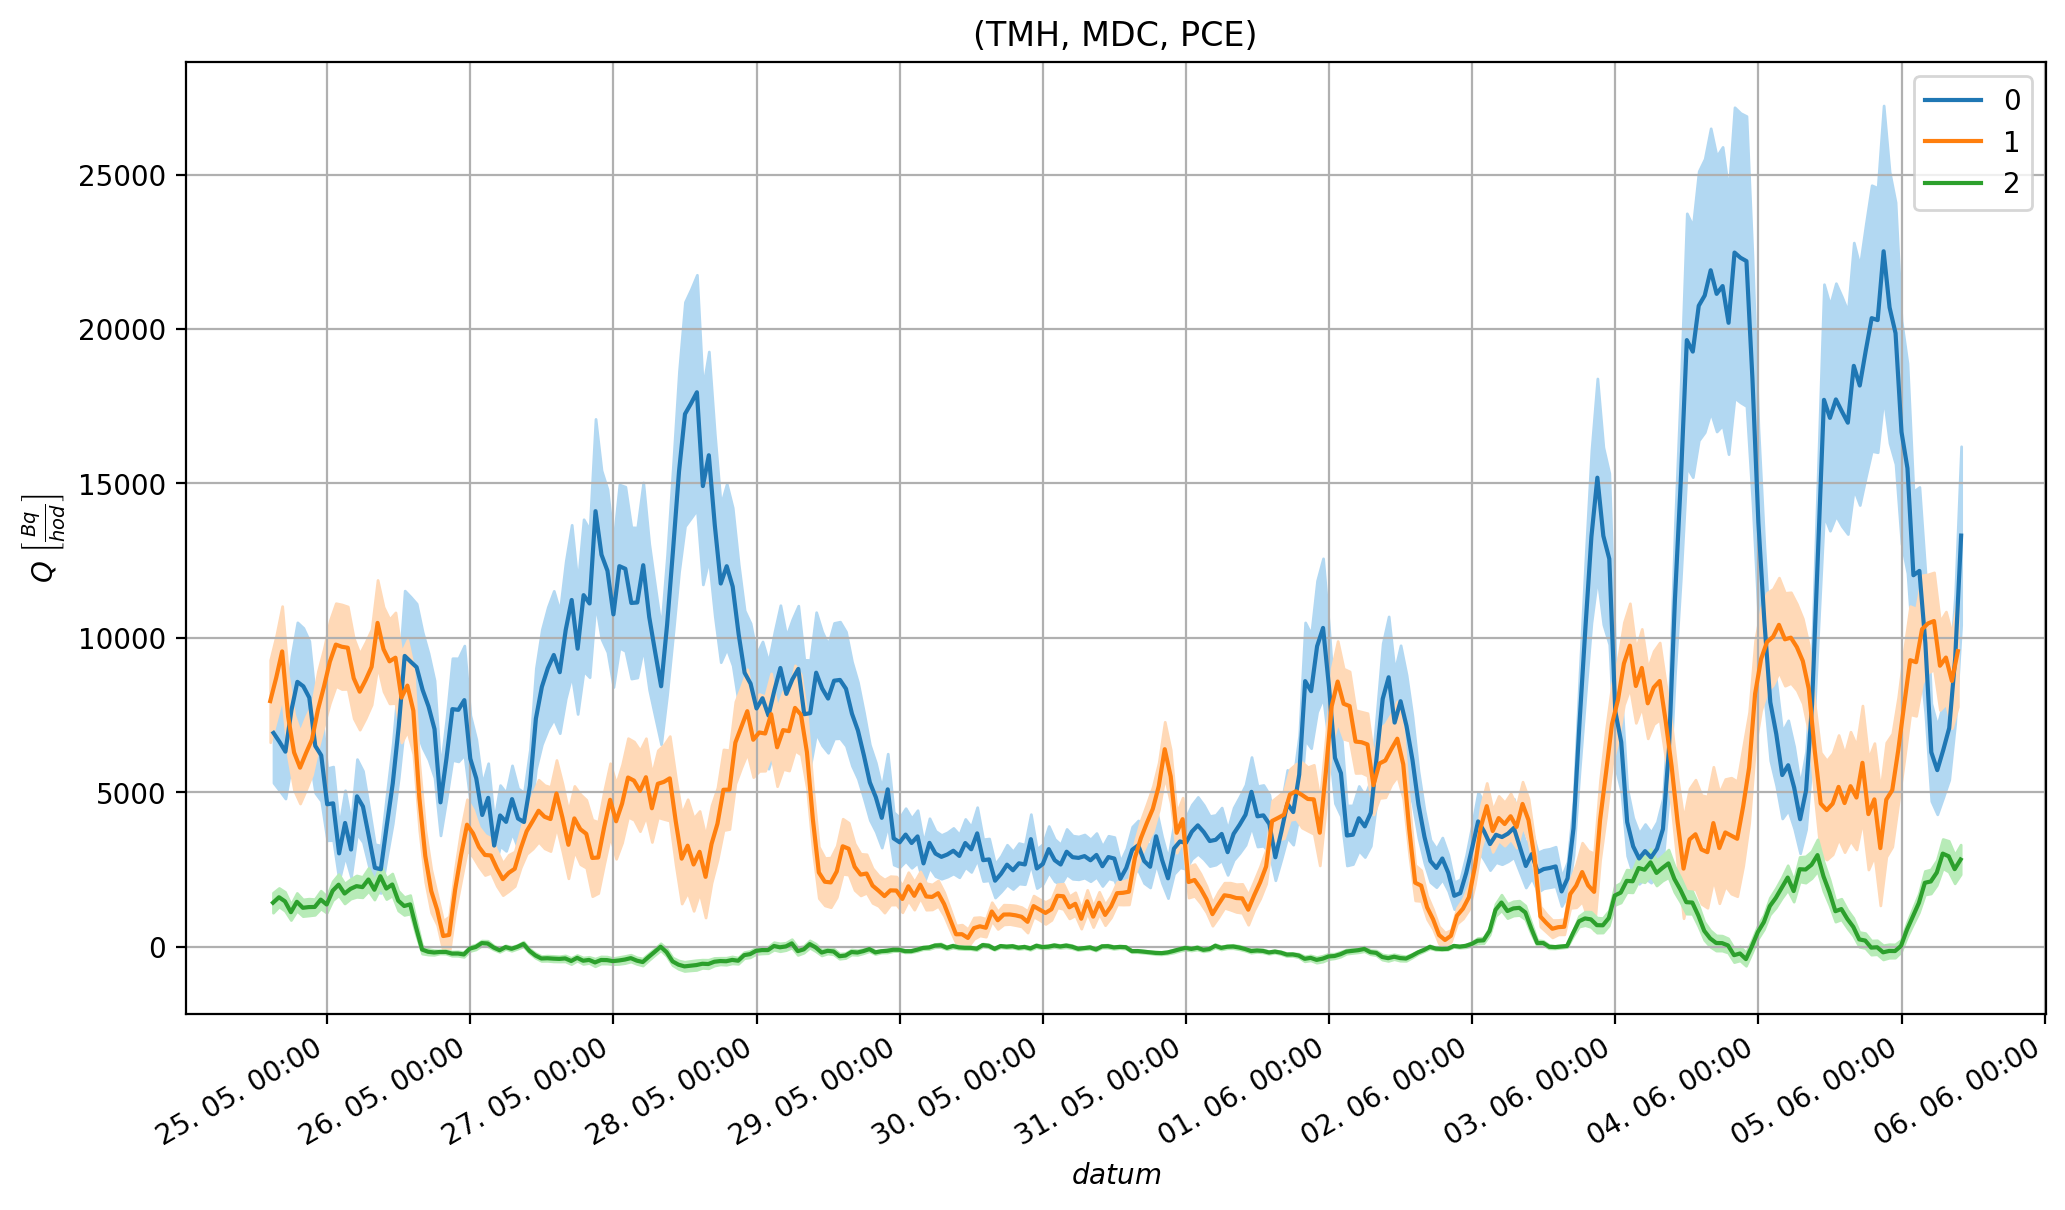
\includegraphics[width=\textwidth]{skala75/prisuny1.png}
    \caption{Určený časový vývoj přísunů radonu do jednotlivých podlaží. Nad obrázkem je uvedena kombinace tří použitých indikačních plynů. Oblasti označené zesvětlenou barvou značí nejistotu přísunů radonu při faktoru pokrytí $k=1$.}
    \label{fig:skala75_prisuny1}
\end{figure}
\begin{table}[H]
    \centering
    \caption{Statistiky vypočítaných přísunů radonu $Q$ do jednotlivých podlaží při stejné kombinaci použitých plynů jako v obr. nad touto tabulkou.}
    \label{tab:skala75_prisuny1}
    \begin{tabular}{lrrr}
\toprule
{} &  $Q_0$ $\left[\si{\frac{Bq}{m^3\cdot hod}}\right]$ &  $Q_1$ $\left[\si{\frac{Bq}{m^3\cdot hod}}\right]$ &  $Q_2$ $\left[\si{\frac{Bq}{m^3\cdot hod}}\right]$ \\
\midrule
count &                                                284 &                                                284 &                                                284 \\
mean  &                                                337 &                                                237 &                                                 19 \\
std   &                                                270 &                                                157 &                                                 84 \\
min   &                                                 15 &                                                -85 &                                               -269 \\
25%   &                                                137 &                                                102 &                                                -19 \\
50%   &                                                222 &                                                237 &                                                 -2 \\
75%   &                                                449 &                                                352 &                                                 29 \\
max   &                                               1161 &                                                891 &                                                371 \\
\bottomrule
\end{tabular}

\end{table}

\begin{figure}[H]
    \centering
    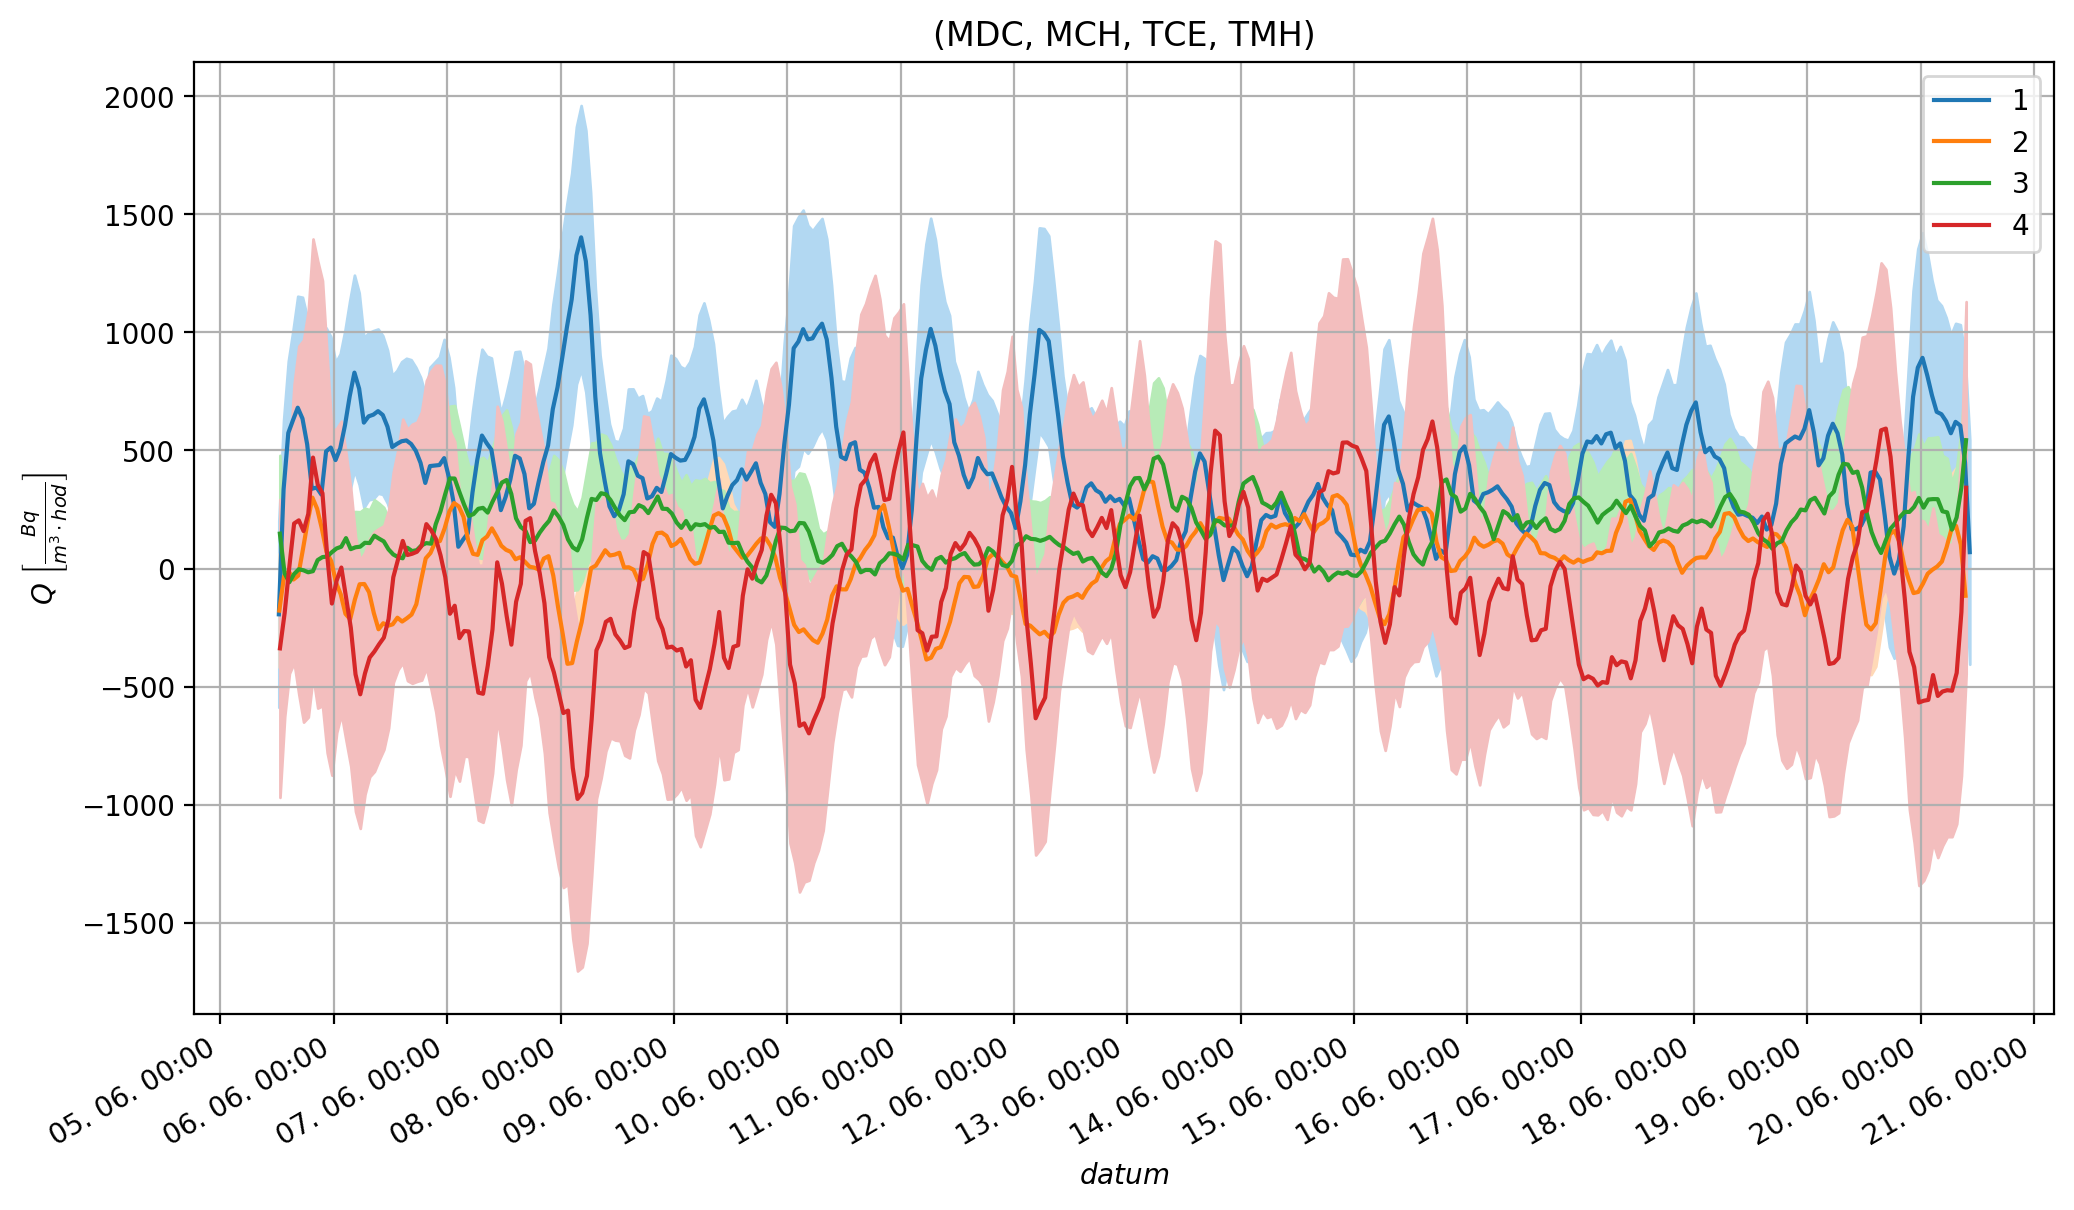
\includegraphics[width=\textwidth]{skala75/prisuny2.png}
    \caption{Určený časový vývoj přísunů radonu do jednotlivých podlaží. Nad obrázkem je uvedena kombinace tří použitých indikačních plynů. Oblasti označené zesvětlenou barvou značí nejistotu přísunů radonu při faktoru pokrytí $k=1$.}
    \label{fig:skala75_prisuny2}
\end{figure}
\begin{table}[H]
    \centering
    \caption{Statistiky vypočítaných přísunů radonu $Q$ do jednotlivých podlaží při stejné kombinaci použitých indikačních plynů jako v obr. nad touto tabulkou.}
    \label{tab:skala75_prisuny2}
    \begin{tabular}{lrrr}
\toprule
{} &  $Q_0$ $\left[\si{\frac{Bq}{hod}}\right]$ &  $Q_1$ $\left[\si{\frac{Bq}{hod}}\right]$ &  $Q_2$ $\left[\si{\frac{Bq}{hod}}\right]$ \\
\midrule
count &                                       284 &                                       284 &                                       284 \\
mean  &                                     12509 &                                     29052 &                                      4320 \\
%std   &                                     10164 &                                     15971 &                                     10993 \\
min   &                                     -1305 &                                      2758 &                                     -7217 \\
25\%   &                                      5053 &                                     13800 &                                     -2574 \\
50\%   &                                      8450 &                                     29570 &                                      -410 \\
75\%   &                                     16517 &                                     41212 &                                     10192 \\
max   &                                     42325 &                                     61230 &                                     36875 \\
\bottomrule
\end{tabular}

\end{table}

\begin{figure}[H]
    \centering
    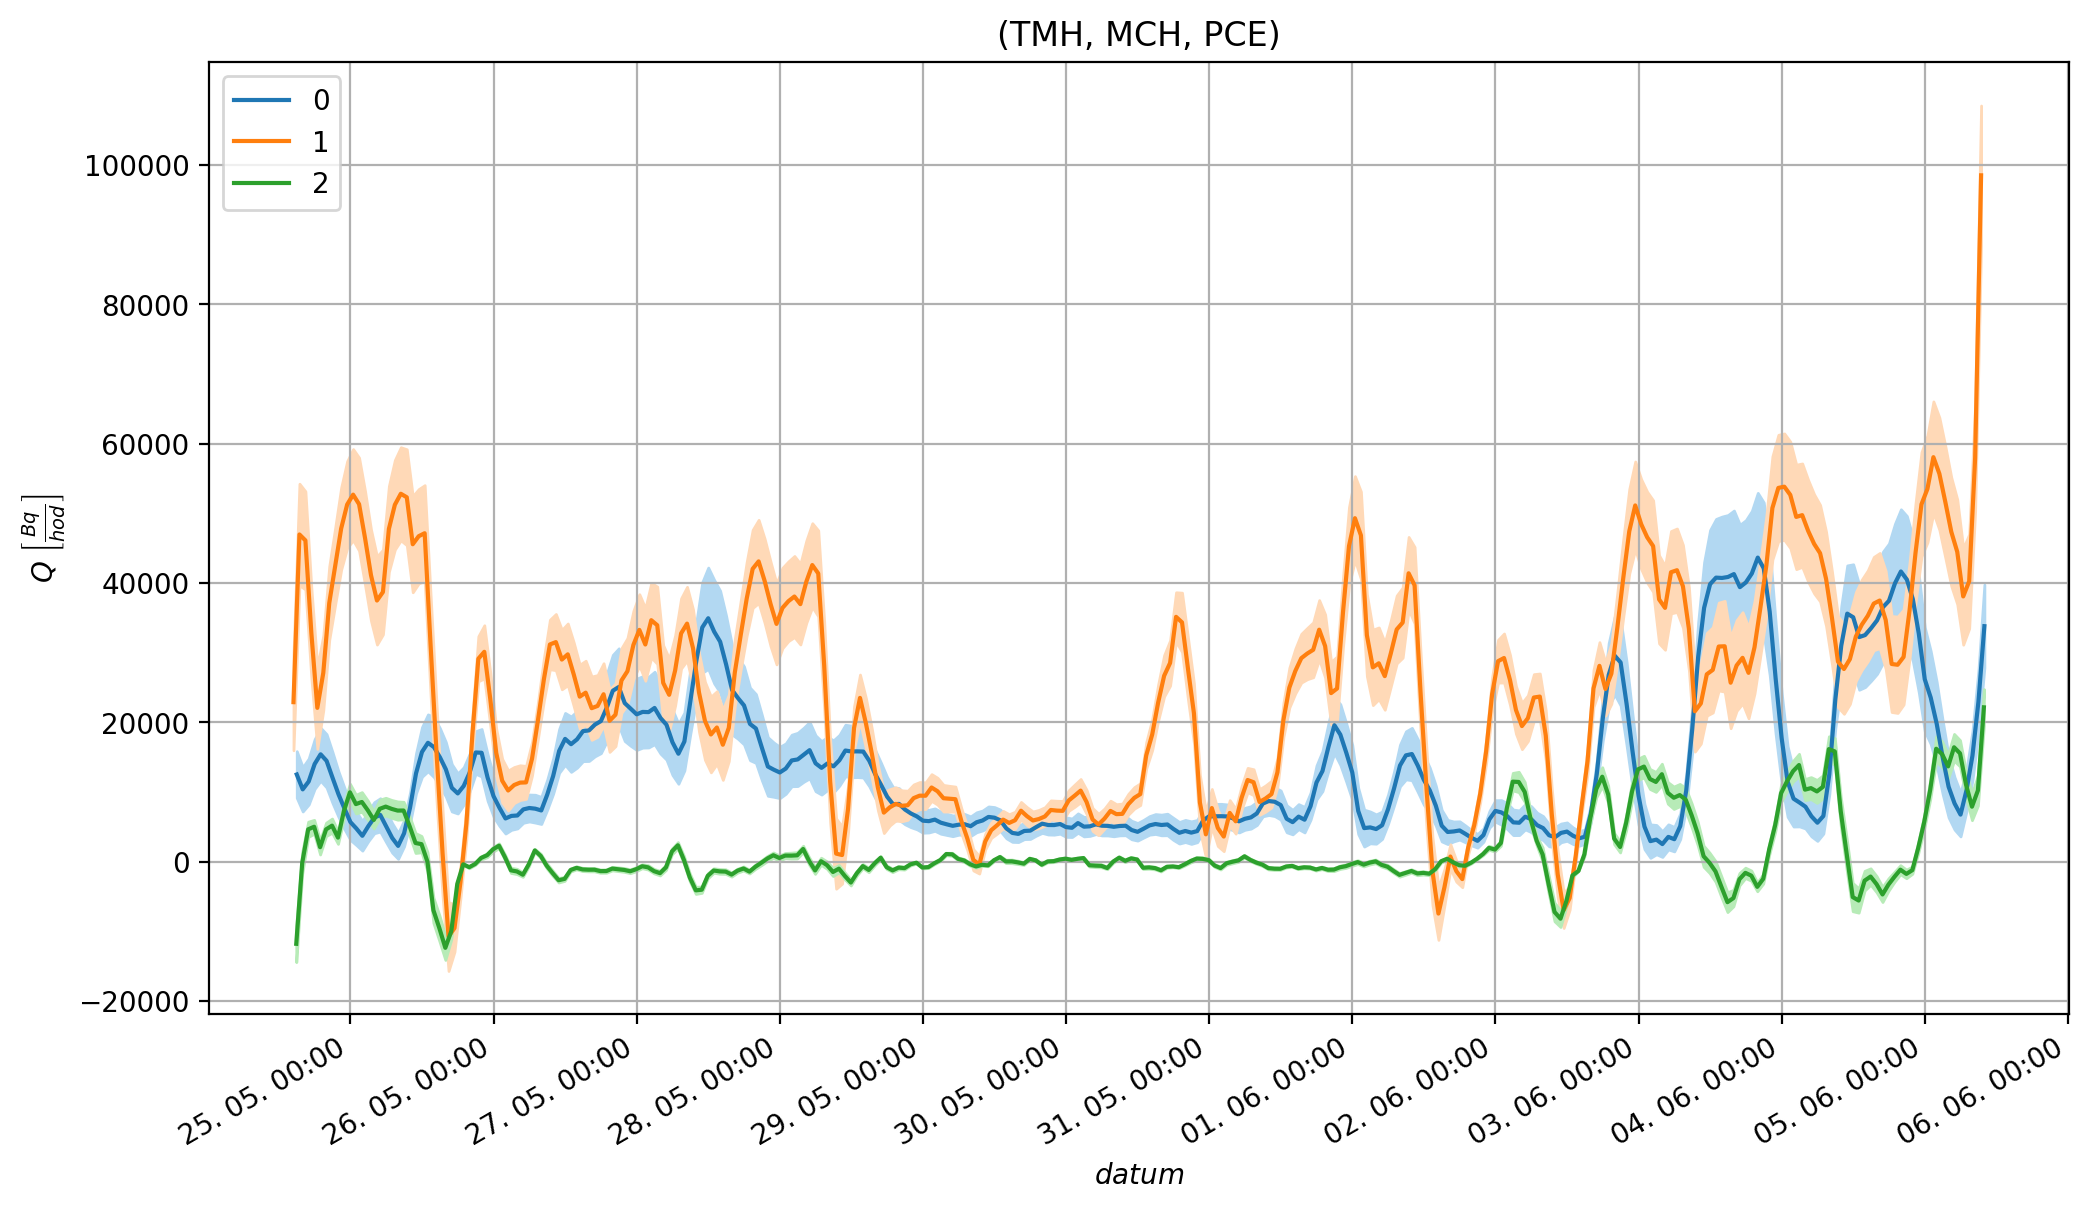
\includegraphics[width=\textwidth]{skala75/prisuny3.png}
    \caption{Určený časový vývoj přísunů radonu do jednotlivých podlaží. Nad obrázkem je uvedena kombinace tří použitých indikačních plynů. Oblasti označené zesvětlenou barvou značí nejistotu přísunů radonu při faktoru pokrytí $k=1$.}
    \label{fig:skala75_prisuny3}
\end{figure}
\begin{table}[H]
    \centering
    \caption{Statistiky vypočítaných přísunů radonu $Q$ do jednotlivých podlaží při stejné kombinaci použitých indikačních plynů jako v obr. nad touto tabulkou.}
    \label{tab:skala75_prisuny3}
    \begin{tabular}{lrrr}
\toprule
{} &  $Q_0$ $\left[\si{\frac{Bq}{hod}}\right]$ &  $Q_1$ $\left[\si{\frac{Bq}{hod}}\right]$ &  $Q_2$ $\left[\si{\frac{Bq}{hod}}\right]$ \\
\midrule
count &                                       284 &                                       284 &                                       284 \\
mean  &                                     13429 &                                     24771 &                                      1333 \\
std   &                                     10114 &                                     14050 &                                      2973 \\
min   &                                      2390 &                                      2315 &                                     -1709 \\
25%   &                                      5647 &                                     11702 &                                      -535 \\
50%   &                                      9781 &                                     24454 &                                       -12 \\
75%   &                                     17323 &                                     35419 &                                      2907 \\
max   &                                     42770 &                                     53869 &                                     10103 \\
\bottomrule
\end{tabular}

\end{table}

\begin{figure}[H]
    \centering
    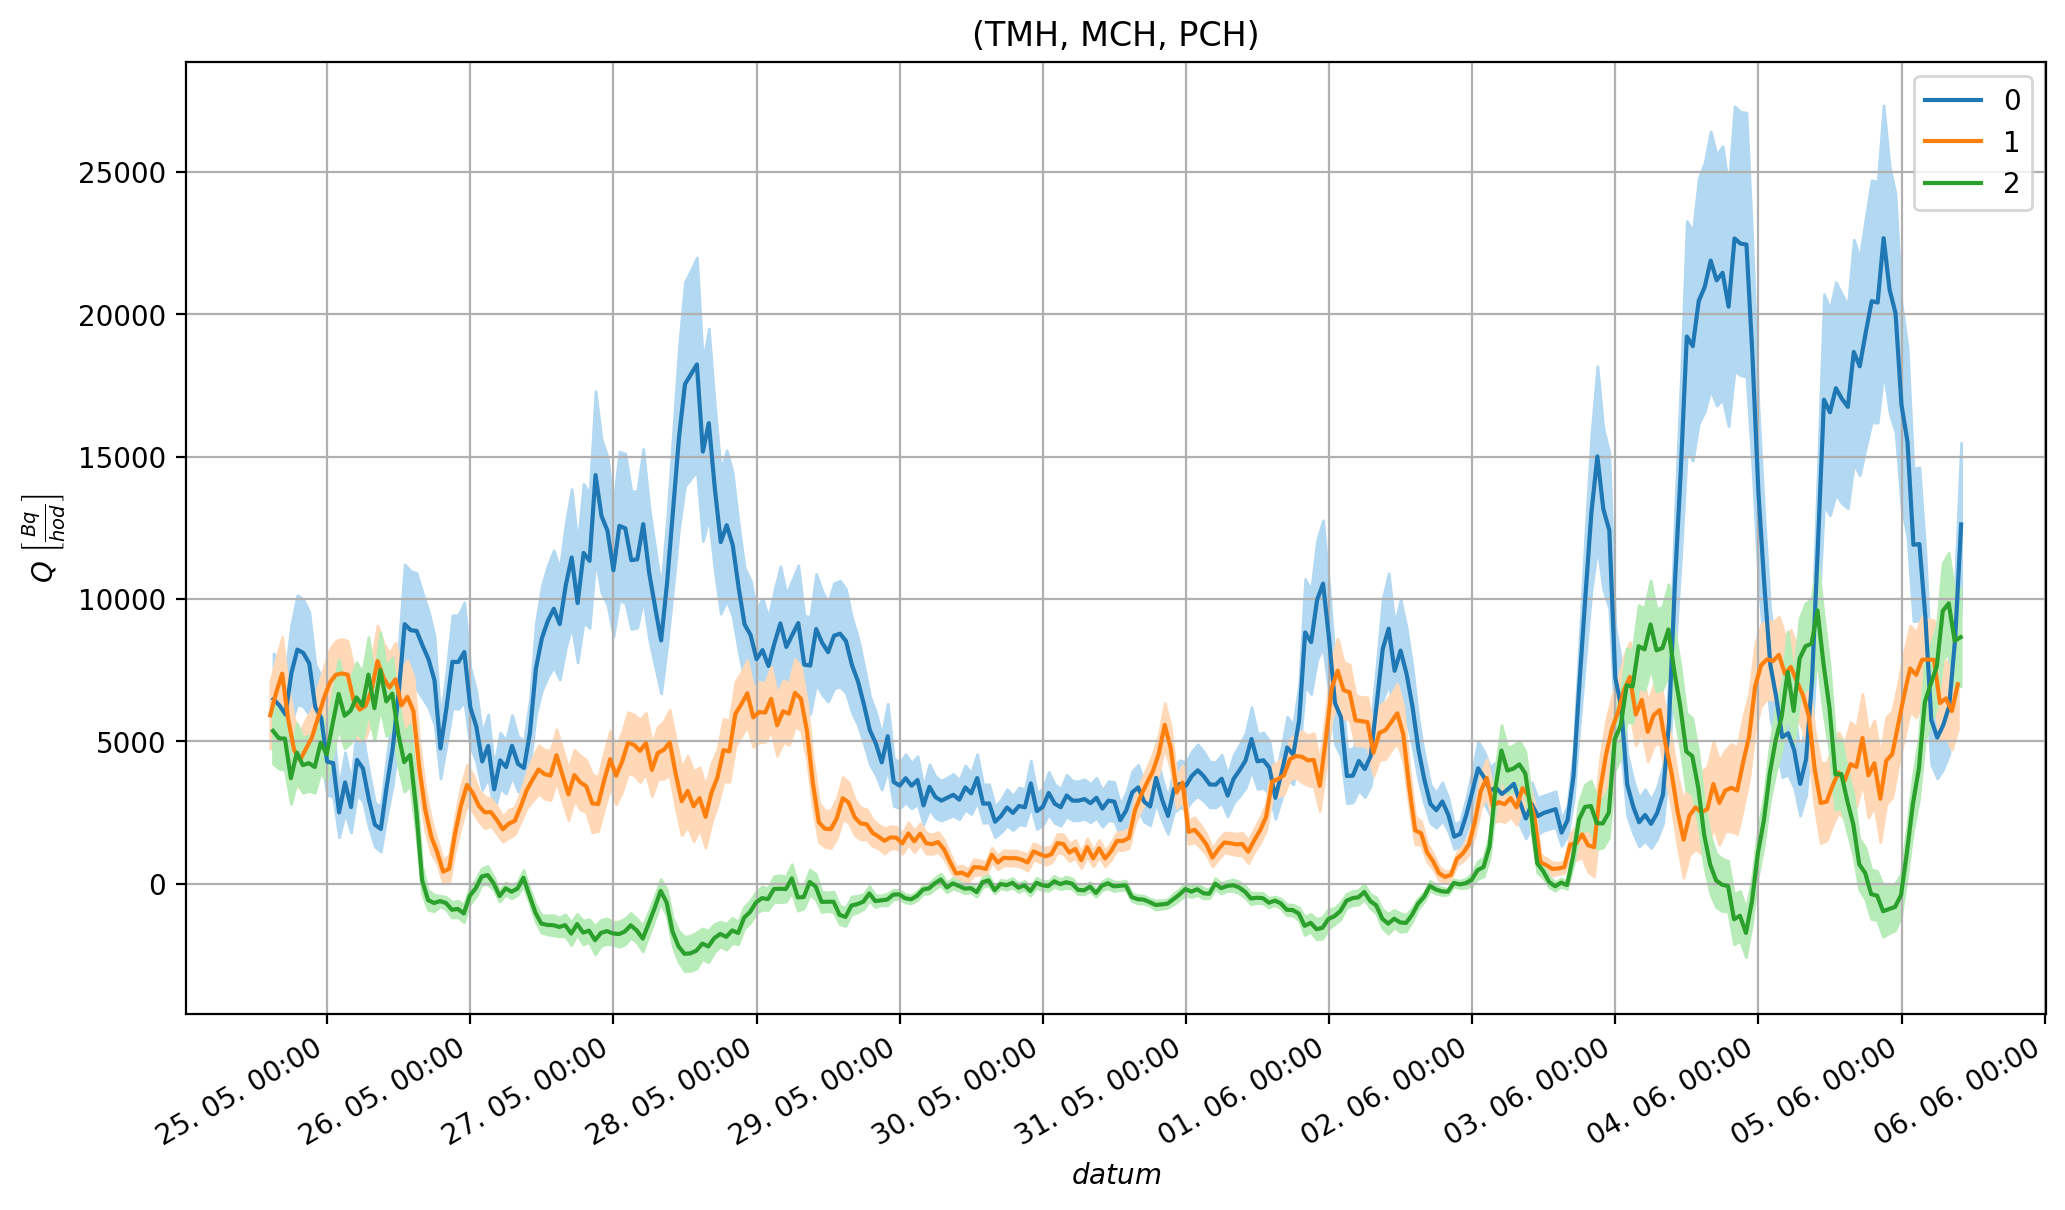
\includegraphics[width=\textwidth]{skala75/prisuny4.png}
    \caption{Určený časový vývoj přísunů radonu do jednotlivých podlaží. Nad obrázkem je uvedena kombinace tří použitých indikačních plynů. Oblasti označené zesvětlenou barvou značí nejistotu přísunů radonu při faktoru pokrytí $k=1$.}
    \label{fig:skala75_prisuny4}
\end{figure}
\begin{table}[H]
    \centering
    \caption{Statistiky vypočítaných přísunů radonu $Q$ do jednotlivých podlaží při stejné kombinaci použitých indikačních plynů jako v obr. nad touto tabulkou.}
    \label{tab:skala75_prisuny4}
    \begin{tabular}{lrrr}
\toprule
{} &  $Q_0$ $\left[\si{\frac{Bq}{hod}}\right]$ &  $Q_1$ $\left[\si{\frac{Bq}{hod}}\right]$ &  $Q_2$ $\left[\si{\frac{Bq}{hod}}\right]$ \\
\midrule
count &                                       284 &                                       284 &                                       284 \\
mean  &                                     12921 &                                     24194 &                                      4807 \\
%std   &                                     10215 &                                     13297 &                                     11131 \\
min   &                                      -501 &                                      2305 &                                     -6720 \\
25\%   &                                      5361 &                                     11493 &                                     -2236 \\
50\%   &                                      8950 &                                     24629 &                                      -191 \\
75\%   &                                     17045 &                                     34319 &                                     10881 \\
max   &                                     42783 &                                     50985 &                                     37529 \\
\bottomrule
\end{tabular}

\end{table}

\begin{figure}[H]
    \centering
    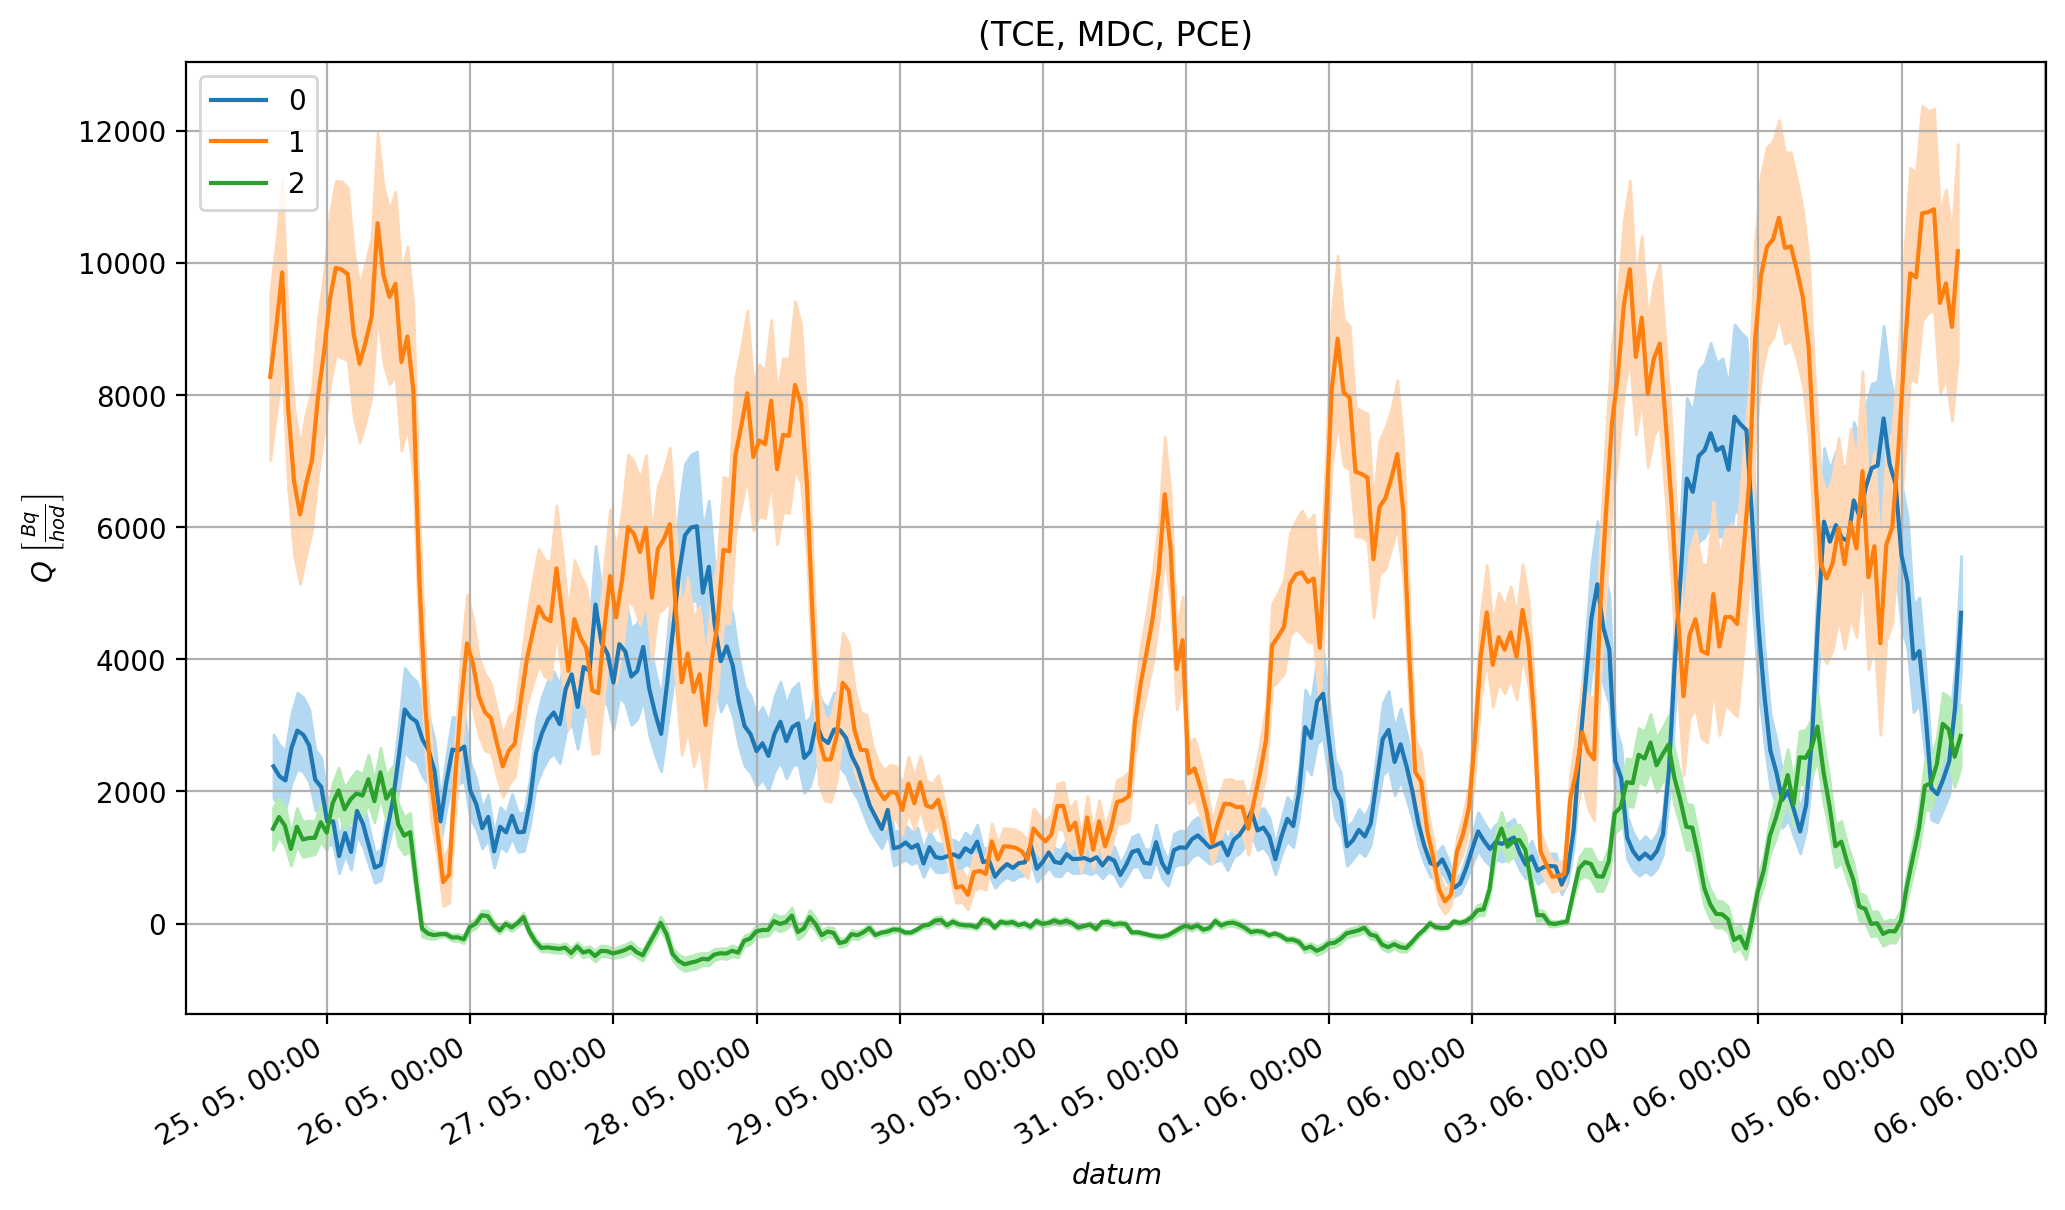
\includegraphics[width=\textwidth]{skala75/prisuny5.png}
    \caption{Určený časový vývoj přísunů radonu do jednotlivých podlaží. Nad obrázkem je uvedena kombinace tří použitých indikačních plynů. Oblasti označené zesvětlenou barvou značí nejistotu přísunů radonu při faktoru pokrytí $k=1$.}
    \label{fig:skala75_prisuny5}
\end{figure}
\begin{table}[H]
    \centering
    \caption{Statistiky vypočítaných přísunů radonu $Q$ do jednotlivých podlaží při stejné kombinaci použitých indikačních plynů jako v obr. nad touto tabulkou.}
    \label{tab:skala75_prisuny5}
    \begin{tabular}{lrrr}
\toprule
{} &  $Q_0$ $\left[\si{\frac{Bq}{m^3\cdot hod}}\right]$ &  $Q_1$ $\left[\si{\frac{Bq}{m^3\cdot hod}}\right]$ &  $Q_2$ $\left[\si{\frac{Bq}{m^3\cdot hod}}\right]$ \\
\midrule
count &                                                284 &                                                284 &                                                284 \\
mean  &                                                113 &                                                250 &                                                 19 \\
%std   &                                                116 &                                                160 &                                                 85 \\
min   &                                                -85 &                                                -78 &                                               -269 \\
25\%   &                                                 37 &                                                111 &                                                -20 \\
50\%   &                                                 74 &                                                255 &                                                 -2 \\
75\%   &                                                161 &                                                369 &                                                 29 \\
max   &                                                528 &                                                913 &                                                371 \\
\bottomrule
\end{tabular}

\end{table}

\begin{figure}[H]
    \centering
    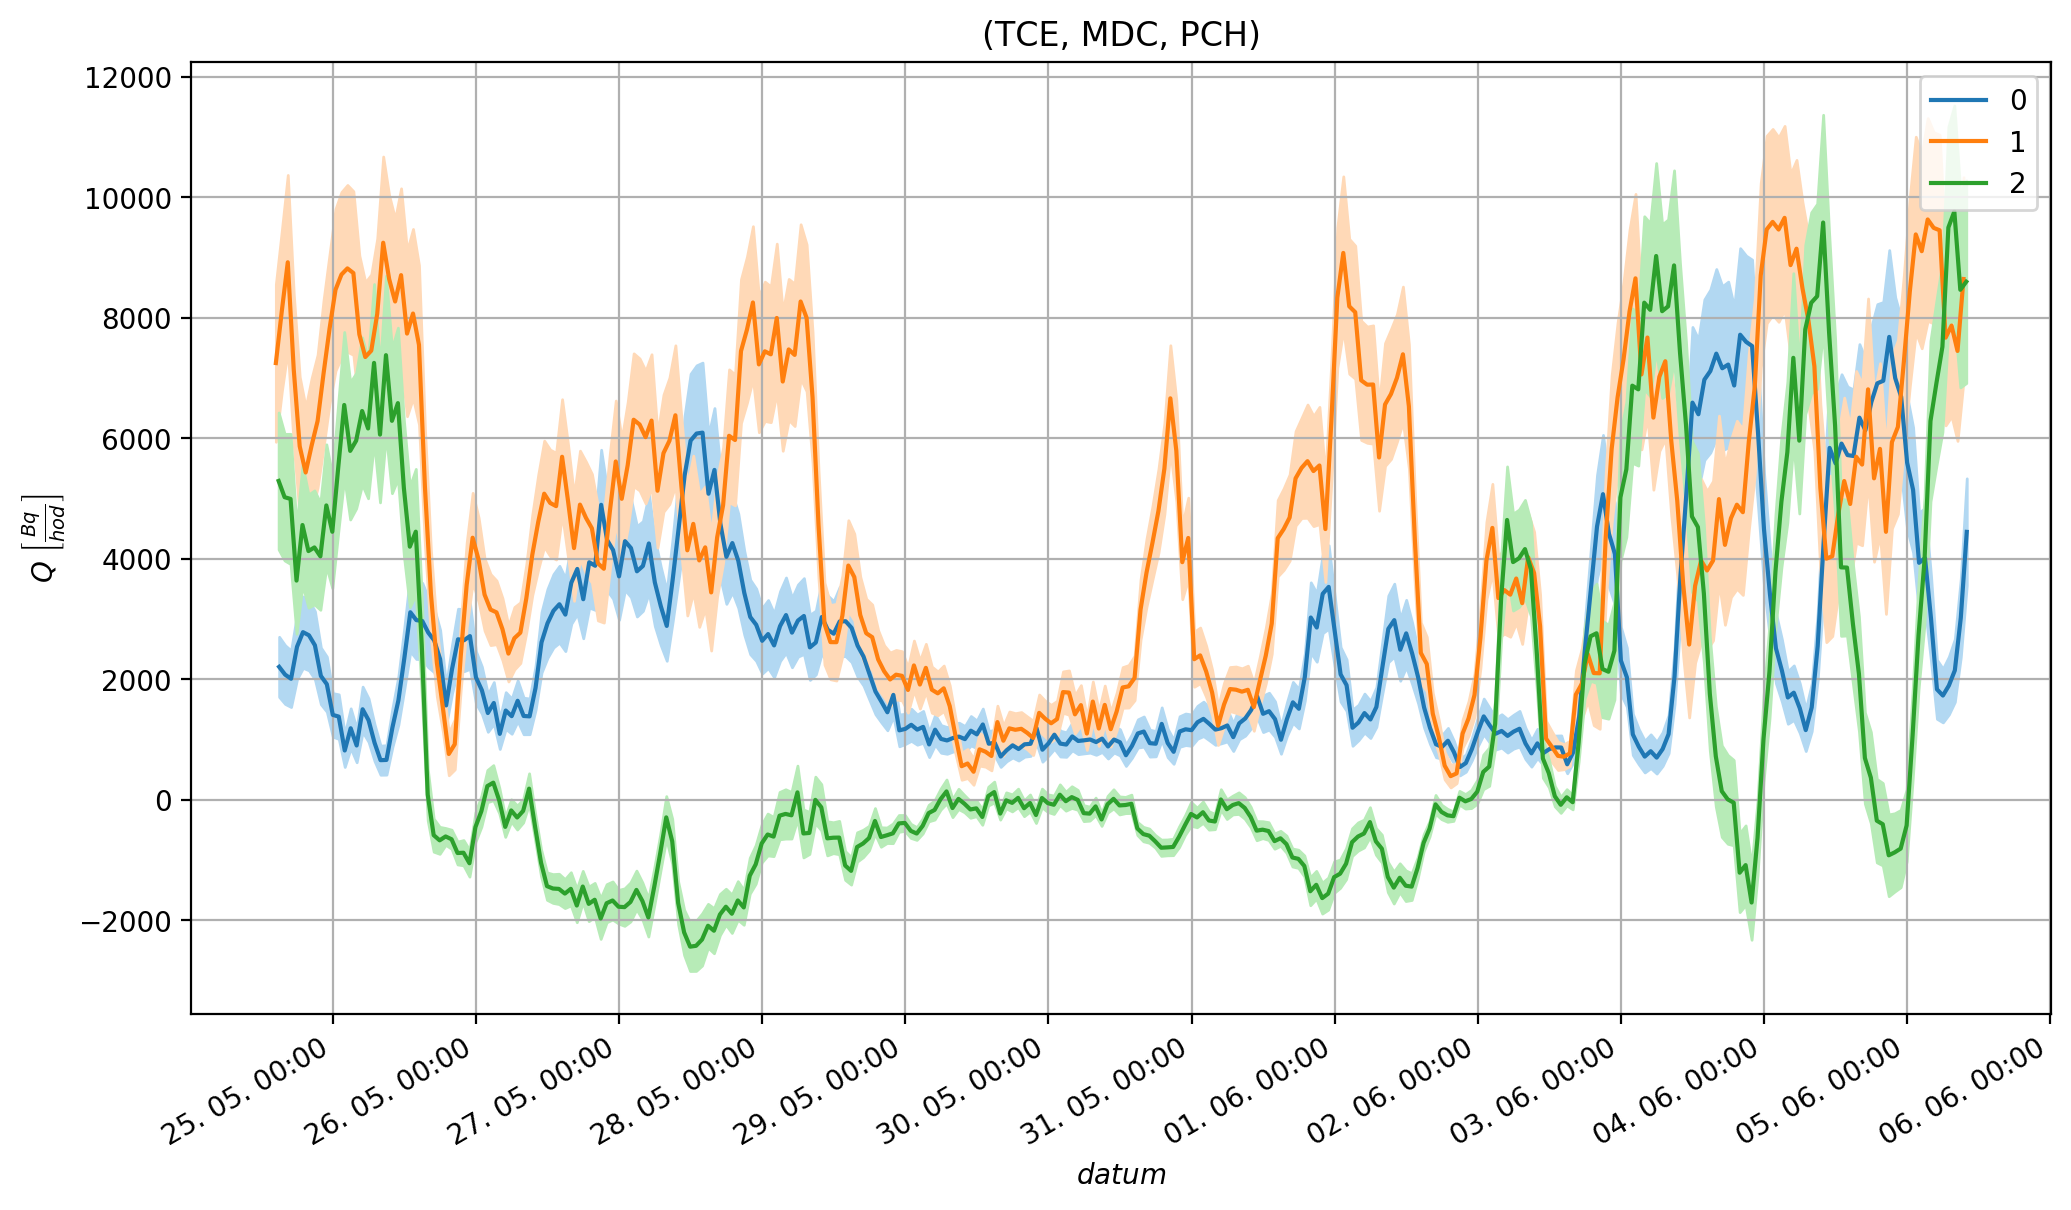
\includegraphics[width=\textwidth]{skala75/prisuny6.png}
    \caption{Určený časový vývoj přísunů radonu do jednotlivých podlaží. Nad obrázkem je uvedena kombinace tří použitých indikačních plynů. Oblasti označené zesvětlenou barvou značí nejistotu přísunů radonu při faktoru pokrytí $k=1$.}
    \label{fig:skala75_prisuny6}
\end{figure}
\begin{table}[H]
    \centering
    \caption{Statistiky vypočítaných přísunů radonu $Q$ do jednotlivých podlaží při stejné kombinaci použitých indikačních plynů jako v obr. nad touto tabulkou.}
    \label{tab:skala75_prisuny6}
    \begin{tabular}{lrrr}
\toprule
{} &  $Q_0$ $\left[\si{\frac{Bq}{hod}}\right]$ &  $Q_1$ $\left[\si{\frac{Bq}{hod}}\right]$ &  $Q_2$ $\left[\si{\frac{Bq}{hod}}\right]$ \\
\midrule
count &                                       284 &                                       284 &                                       284 \\
mean  &                                      4233 &                                     30807 &                                      4359 \\
%std   &                                      4526 &                                     19577 &                                     12339 \\
min   &                                     -4010 &                                    -10346 &                                    -16011 \\
25\%   &                                      1203 &                                     13494 &                                     -3348 \\
50\%   &                                      2855 &                                     31079 &                                      -669 \\
75\%   &                                      6299 &                                     45500 &                                      8645 \\
max   &                                     19350 &                                    110431 &                                     49402 \\
\bottomrule
\end{tabular}

\end{table}

\begin{figure}[H]
    \centering
    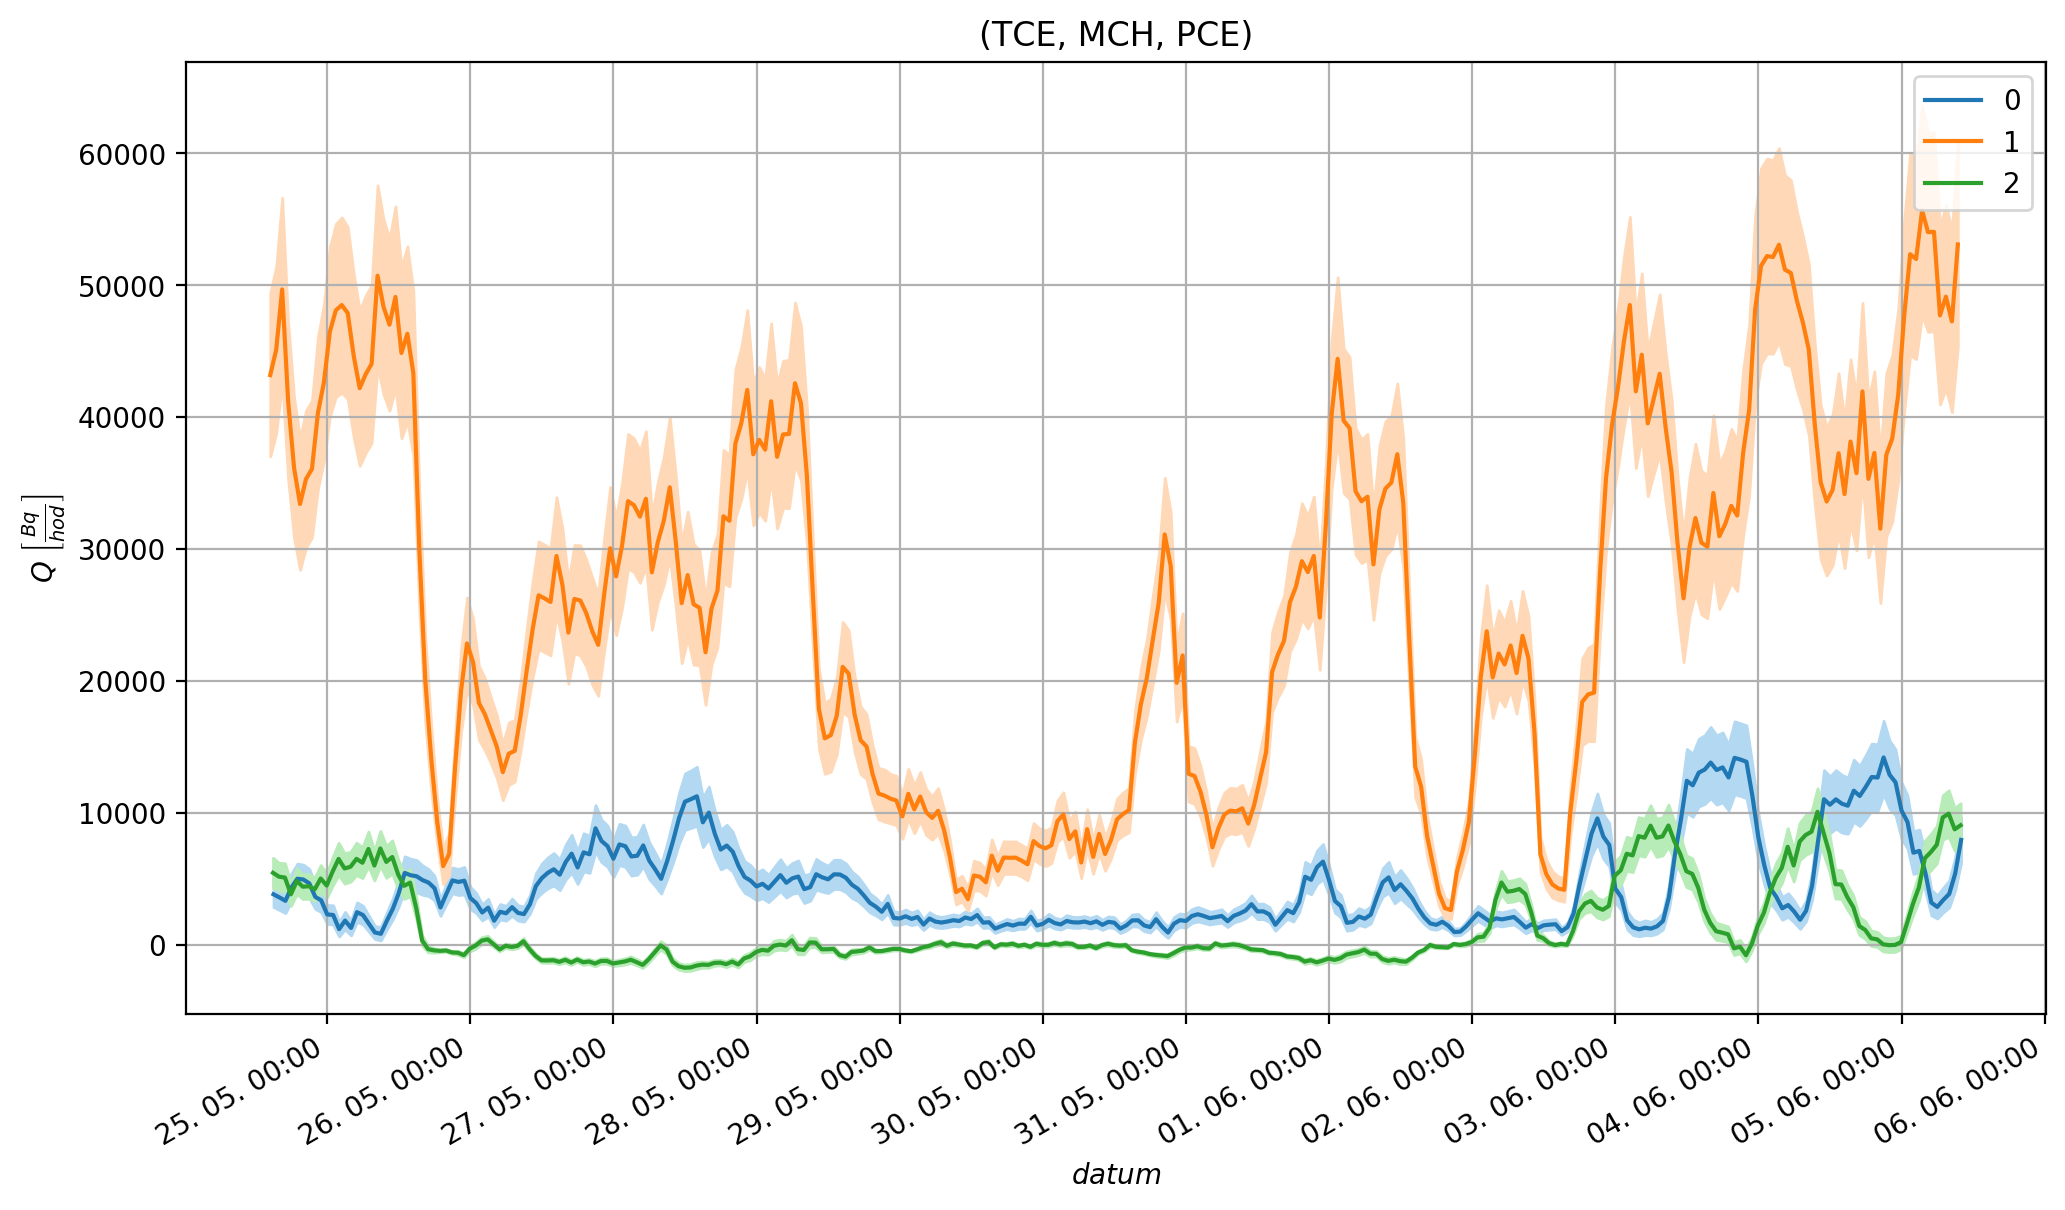
\includegraphics[width=\textwidth]{skala75/prisuny7.png}
    \caption{Určený časový vývoj přísunů radonu do jednotlivých podlaží. Nad obrázkem je uvedena kombinace tří použitých indikačních plynů. Oblasti označené zesvětlenou barvou značí nejistotu přísunů radonu při faktoru pokrytí $k=1$.}
    \label{fig:skala75_prisuny7}
\end{figure}
\begin{table}[H]
    \centering
    \caption{Statistiky vypočítaných přísunů radonu $Q$ do jednotlivých podlaží při stejné kombinaci použitých indikačních plynů jako v obr. nad touto tabulkou.}
    \label{tab:skala75_prisuny7}
    \begin{tabular}{lrrr}
\toprule
{} &  $Q_0$ $\left[\si{\frac{Bq}{hod}}\right]$ &  $Q_1$ $\left[\si{\frac{Bq}{hod}}\right]$ &  $Q_2$ $\left[\si{\frac{Bq}{hod}}\right]$ \\
\midrule
count &                                       284 &                                       284 &                                       284 \\
mean  &                                      4466 &                                     26182 &                                      1325 \\
%std   &                                      3357 &                                     14388 &                                      2973 \\
min   &                                       847 &                                      2646 &                                     -1726 \\
25\%   &                                      1868 &                                     12472 &                                      -540 \\
50\%   &                                      3228 &                                     26241 &                                       -15 \\
75\%   &                                      5735 &                                     37368 &                                      2890 \\
max   &                                     14210 &                                     55660 &                                     10091 \\
\bottomrule
\end{tabular}

\end{table}

\begin{figure}[H]
    \centering
    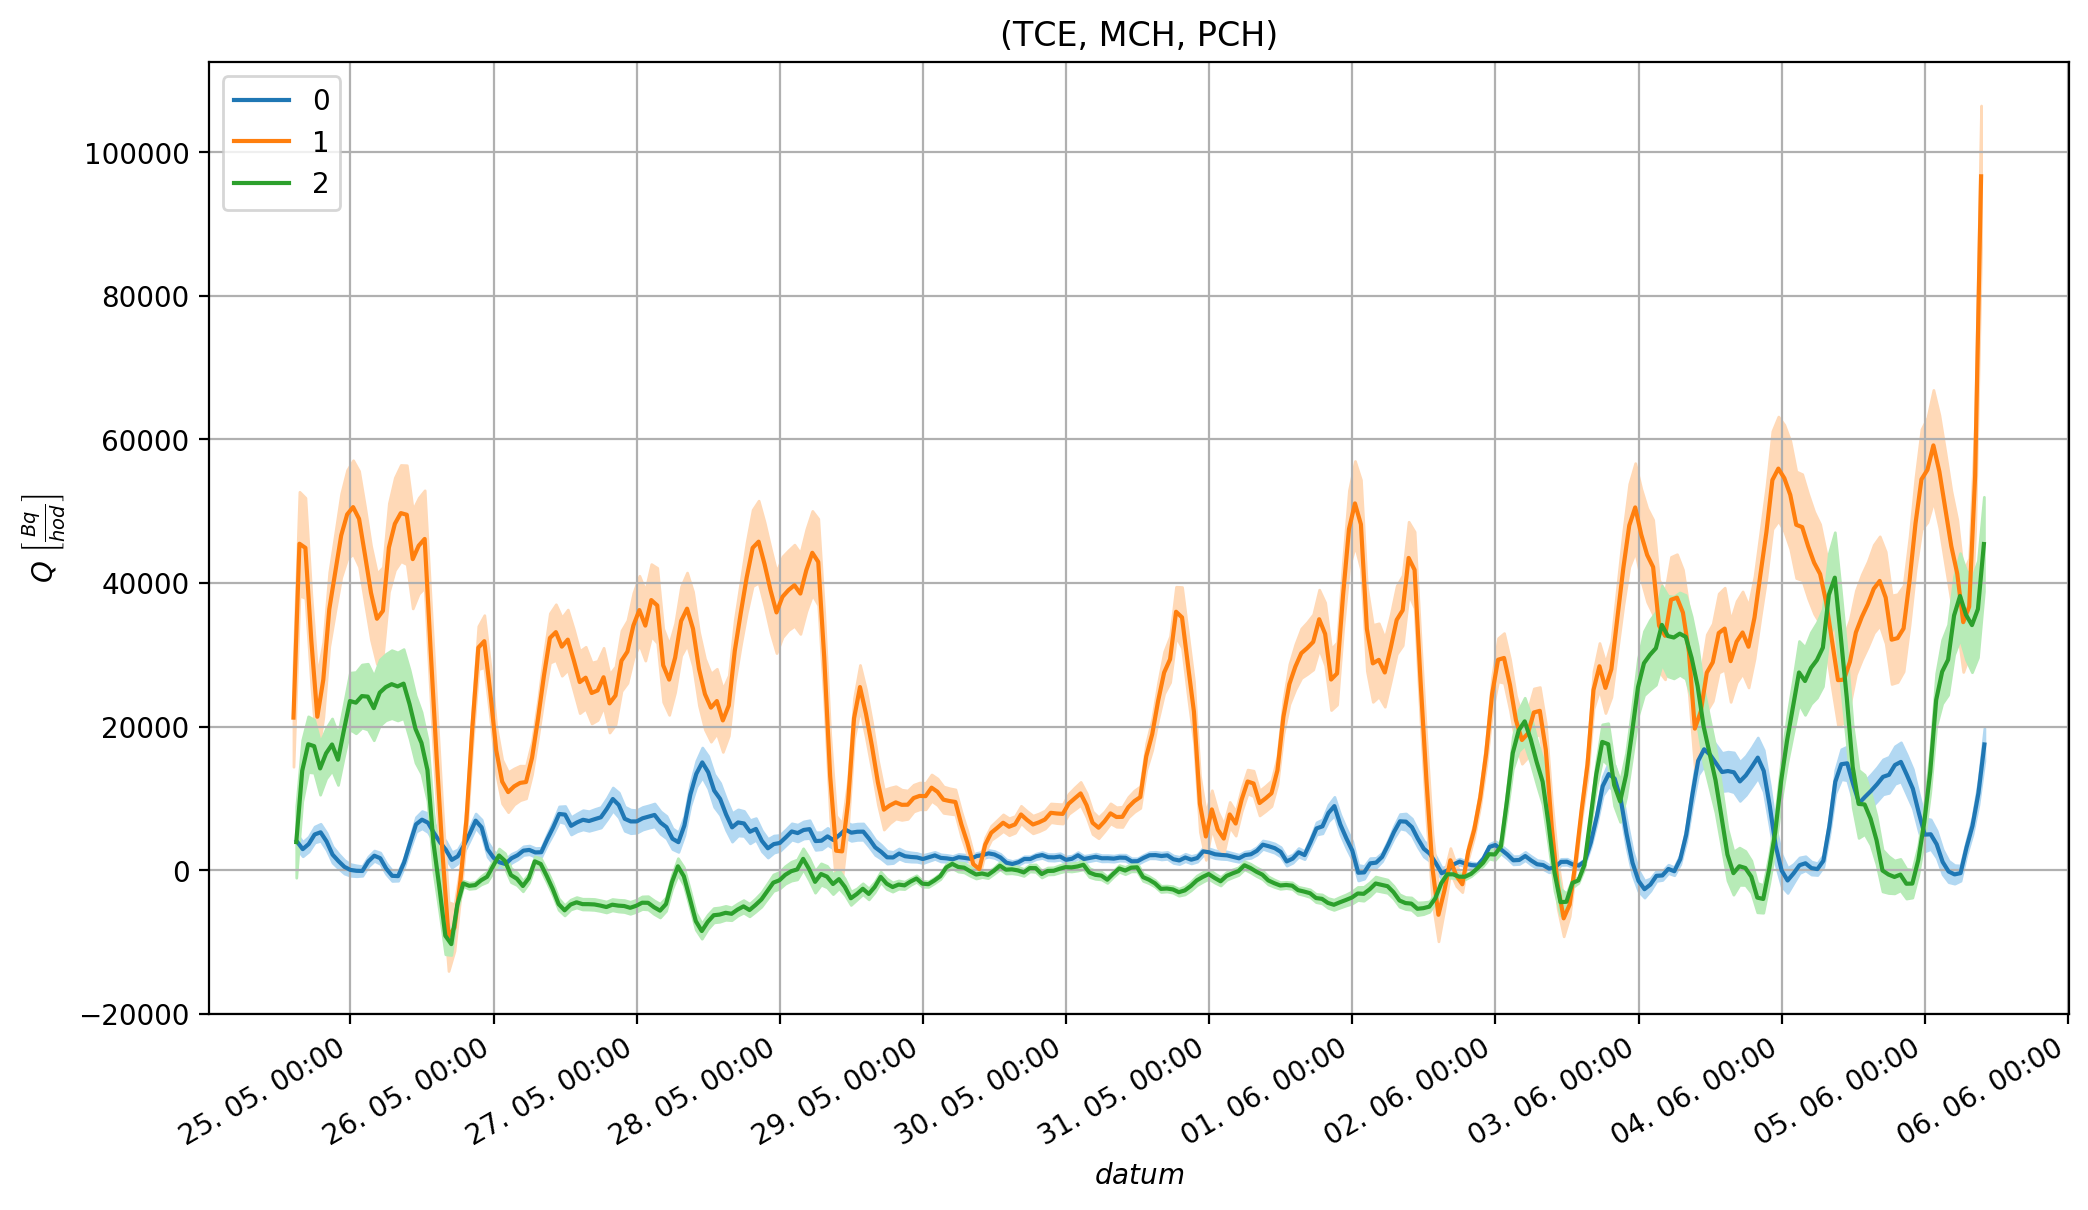
\includegraphics[width=\textwidth]{skala75/prisuny8.png}
    \caption{Určený časový vývoj přísunů radonu do jednotlivých podlaží. Nad obrázkem je uvedena kombinace tří použitých indikačních plynů. Oblasti označené zesvětlenou barvou značí nejistotu přísunů radonu při faktoru pokrytí $k=1$.}
    \label{fig:skala75_prisuny8}
\end{figure}
\begin{table}[H]
    \centering
    \caption{Statistiky vypočítaných přísunů radonu $Q$ do jednotlivých podlaží při stejné kombinaci použitých indikačních plynů jako v obr. nad touto tabulkou.}
    \label{tab:skala75_prisuny8}
    \begin{tabular}{lrrr}
\toprule
{} &  $Q_0$ $\left[\si{\frac{Bq}{m^3\cdot hod}}\right]$ &  $Q_1$ $\left[\si{\frac{Bq}{m^3\cdot hod}}\right]$ &  $Q_2$ $\left[\si{\frac{Bq}{m^3\cdot hod}}\right]$ \\
\midrule
count &                                                284 &                                                284 &                                                284 \\
mean  &                                               2536 &                                               3929 &                                               1148 \\
std   &                                               1795 &                                               2200 &                                               3007 \\
min   &                                                545 &                                                337 &                                              -2379 \\
25\%   &                                               1145 &                                               1866 &                                               -643 \\
50\%   &                                               1934 &                                               3842 &                                               -135 \\
75\%   &                                               3243 &                                               5850 &                                               2588 \\
max   &                                               7736 &                                               8235 &                                               9876 \\
\bottomrule
\end{tabular}

\end{table}

\begin{table}[H]
    \centering
    \caption{Průměrné přísuny radonu souhrně pro všechny kombinace indikačních plynů pro dynamické vyhodnocení.}
    \label{tab:skala75_prisunyDynamicky}
   \begin{tabular}{lrrrr}
\toprule
použité tracery & $Q_0$ $\left[\si{\frac{Bq}{m^3\cdot hod}}\right]$ & $Q_1$ $\left[\si{\frac{Bq}{m^3\cdot hod}}\right]$ & $Q_2$ $\left[\si{\frac{Bq}{m^3\cdot hod}}\right]$ & $Q_3$ $\left[\si{\frac{Bq}{m^3\cdot hod}}\right]$ \\
\midrule
(MDC, PCE, TCE, TMH) & 401+/-383 &    9+/-243 &       97+/-163 &                               -100+/-611 \\
(MDC, MCH, TCE, TMH) & 398+/-356 &   29+/-183 &      101+/-158 &                               -103+/-575 \\
\bottomrule
\end{tabular}

\end{table}
\subsubsection{Vyhodnocení v rovnovážném stavu}
\begin{table}[H]
    \centering
    \caption{Průměrné objemové koncentrace radonu naměřené TERA sondami. $\sigma_A$ je nejistota typu A plynoucí ze statistického zpracování naměřených dat, $\sigma_B$ je nejistota typu B plynoucí z nejistoty měřidla a $\sigma$ je kombinovaná nejistota. Při určování přísunů radonu v rovnovážném stavu byla použita pouze nejistota typu B, tj. $\sigma_B$. V posledním sloupci je průměrná citlivost TERA sond vypočtená z naměřených dat (tj. z naměřeného počtu impulzů a naměřeného OAR). Tato citlivost byla použita pro výpočet $\sigma_B$.}
    \label{tab:skala75_OARprumerne}
    \begin{tabular}{llrrrrr}
\toprule
ID sondy&podlaží& OAR [\si{Bq/m^3}]& $\sigma_A$ & $\sigma_B$ &$\sigma$& prům. citlivost $\left[\si{\frac{imp}{hod}/\frac{Bq}{m^3}}\right]$\\ 
\midrule
8  &0 & 458 & 309 & 33 & 311&0,405\\
10 &1 & 789 & 485 & 43 & 487&0,433\\
112&1 & 633 & 282 & 37 & 284&0,464\\
88 &2 & 276 & 356 & 31 & 358&0,296\\
\bottomrule
    \end{tabular}
\end{table}

\begin{table}[H]
    \centering
    \caption{Přísuny radonu určené z průměrných hodnot OAR, tj. jako v rovnovážném měření.}
    \label{tab:skala75_prisunyRovnovazne}
   \begin{tabular}{llll}
\toprule
{} & $Q_0$ $\left[\si{\frac{Bq}{m^3\cdot hod}}\right]$ & $Q_1$ $\left[\si{\frac{Bq}{m^3\cdot hod}}\right]$ & $Q_2$ $\left[\si{\frac{Bq}{m^3\cdot hod}}\right]$ \\
\midrule
(TMH, MDC, PCE) &                                          335+/-90 &                                          236+/-42 &                                            18+/-6 \\
(TMH, MDC, PCH) &                                          323+/-88 &                                          231+/-42 &                                           63+/-24 \\
(TMH, MCH, PCE) &                                          347+/-89 &                                          197+/-36 &                                            19+/-6 \\
(TMH, MCH, PCH) &                                          334+/-87 &                                          192+/-35 &                                           70+/-24 \\
(TCE, MDC, PCE) &                                          111+/-28 &                                          249+/-41 &                                            17+/-6 \\
(TCE, MDC, PCH) &                                          108+/-28 &                                          243+/-41 &                                           62+/-23 \\
(TCE, MCH, PCE) &                                          115+/-26 &                                          208+/-35 &                                            19+/-6 \\
(TCE, MCH, PCH) &                                          111+/-27 &                                          203+/-35 &                                           70+/-23 \\
\bottomrule
\end{tabular}

\end{table}
%\subsection{Přeurčená varianta}

%\begin{table}[H]
    %\centering
    %\caption{Průtoky vzduchu mezi jednotlivými zónami. Vnější prostředí je označeno číslem 4.}
    %\label{tab:skala75Preurcena_prutoky}
    %\begin{tabular}{ll}
\toprule
k12 &  3.0+/-1.9 \\
k13 &  0.7+/-1.9 \\
k21 &  0.2+/-0.7 \\
k23 &  0.3+/-0.7 \\
k31 &  0.1+/-1.3 \\
k32 &  0.6+/-1.3 \\
k14 &  2.9+/-3.3 \\
k24 &  6.9+/-1.3 \\
k34 &  3.1+/-2.2 \\
k41 &      6+/-5 \\
k42 &  3.7+/-2.9 \\
k43 &      3+/-4 \\
\bottomrule
\end{tabular}

%\end{table}
%\begin{table}[H]
    %\centering
    %\caption{Statistiky vypočítaných přísunů radonu $Q$ do jednotlivých zón.}
    %\label{tab:skala75Preurcena_objemy}
    %\begin{tabular}{lrrr}
\toprule
{} &  $Q_0$ $\left[\si{\frac{Bq}{m^3\cdot hod}}\right]$ &  $Q_1$ $\left[\si{\frac{Bq}{m^3\cdot hod}}\right]$ &  $Q_2$ $\left[\si{\frac{Bq}{m^3\cdot hod}}\right]$ \\
\midrule
count &                                                309 &                                                309 &                                                309 \\
mean  &                                                 70 &                                                 34 &                                                 10 \\
std   &                                                134 &                                                156 &                                                101 \\
min   &                                               -991 &                                               -419 &                                               -305 \\
25\\%   &                                                 18 &                                                -14 &                                                -20 \\
50\\%   &                                                 52 &                                                 27 &                                                 -0 \\
75\\%   &                                                109 &                                                 86 &                                                 22 \\
max   &                                                879 &                                               2169 &                                                914 \\
\bottomrule
\end{tabular}

%\end{table}

%\begin{figure}[H]
    %\centering
    %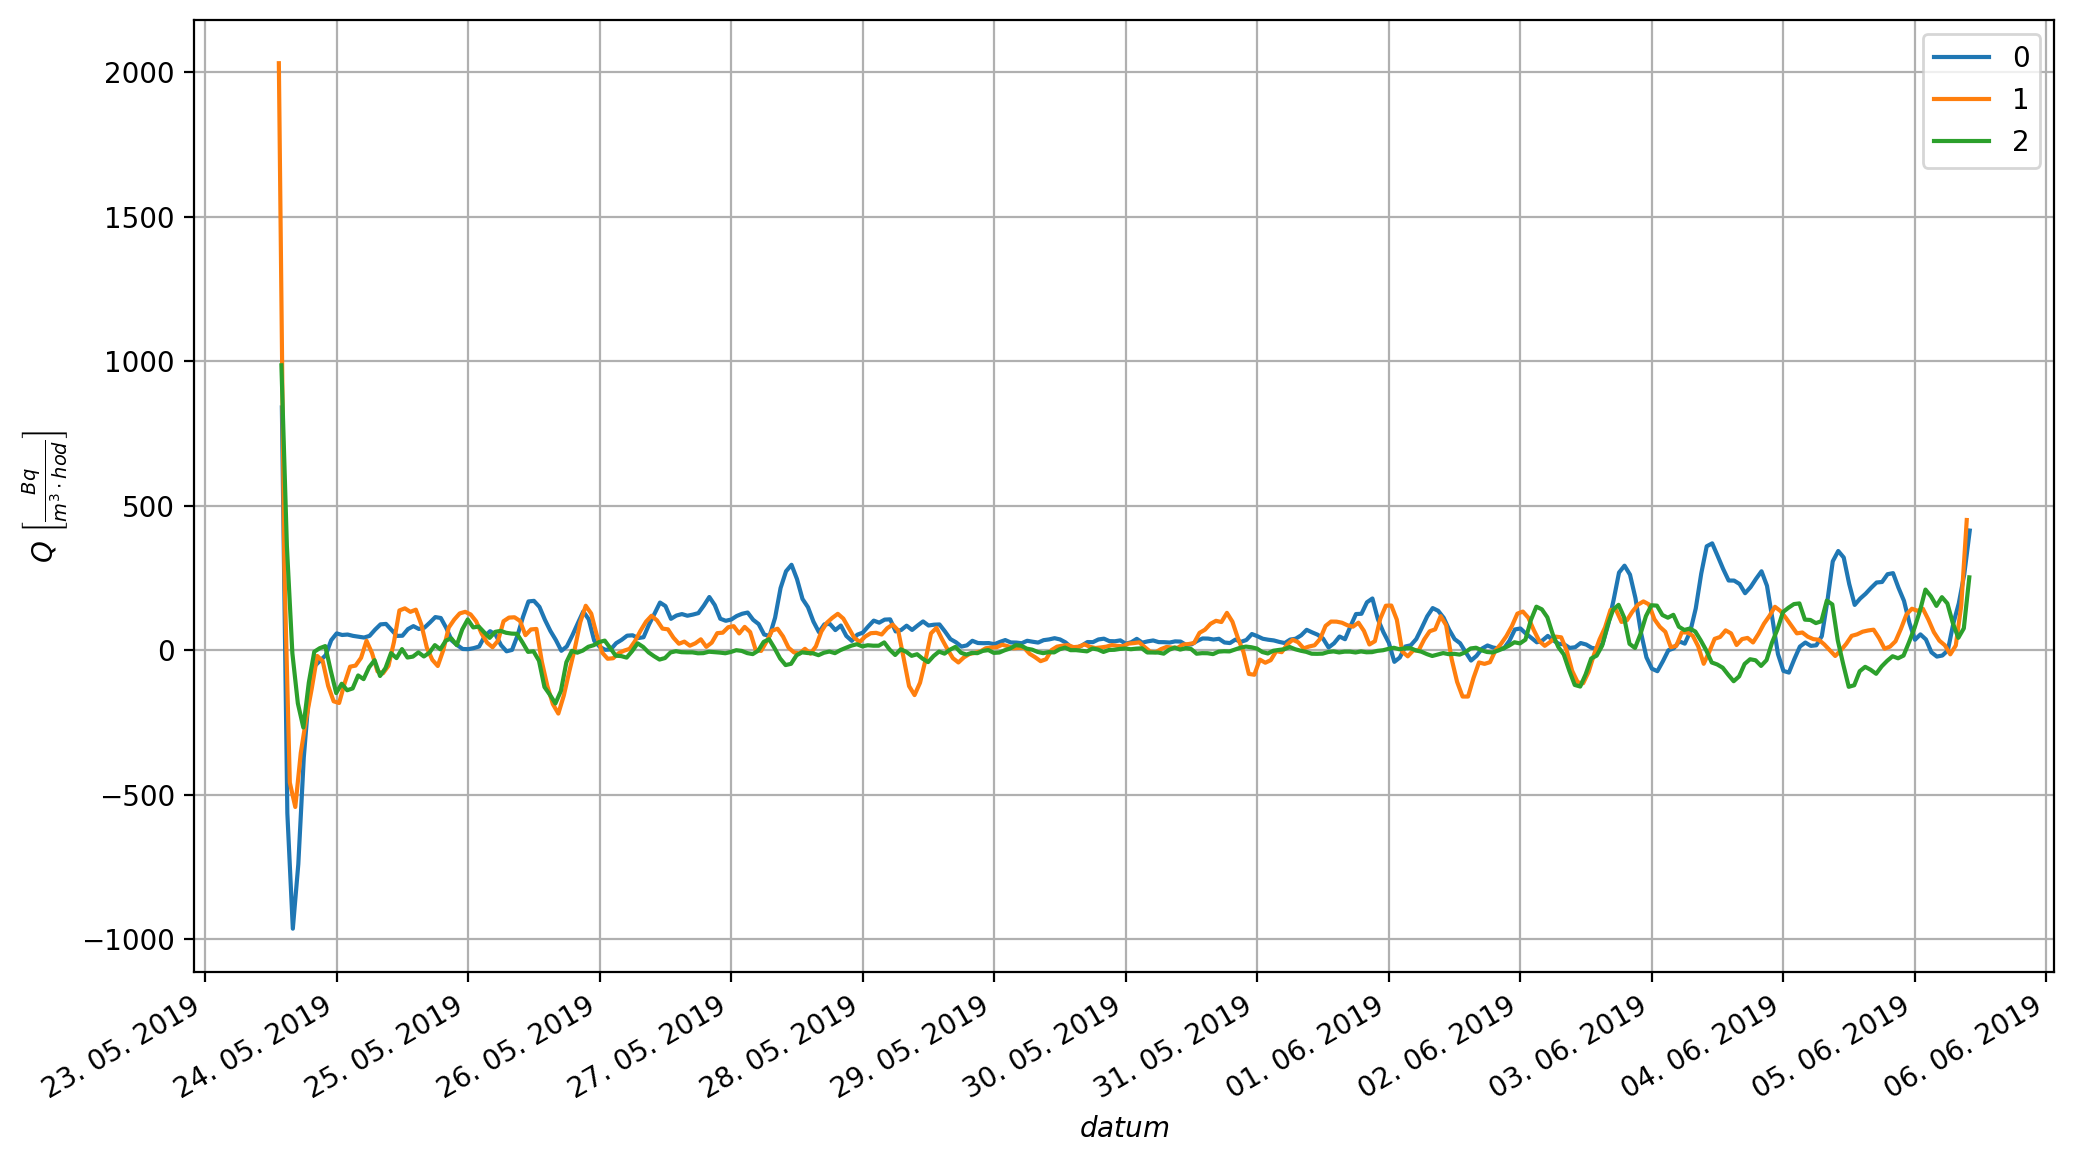
\includegraphics[width=\textwidth]{skala75/prisuny_preurcena.png}
    %\caption{Přísuny radonu. Popisky v legendě značí podlaží.}
    %\label{fig:skala75Preurcena_prisuny}
%\end{figure}

\section{Objekt Hálková 980, Humpolec}
\subsection{Použitá měřidla}
\begin{itemize}
    \setlength\itemsep{0em}
	\item 20 vyvíječů (4x TMH, 4x TCE, 4x MDC, 4x MCH, 4x PCE)
	\item 8 TD detektorů
	\item 4 CANARY monitory
	\item 4 TERA sondy
	\item 3 TESTO měřiče teploty a vlhkosti
	\item 1 zdroj radonu
\end{itemize}

\section{Objekt Anglická 574, Dobřichovice}
\subsection{Použitá měřidla}
\begin{itemize}
    \setlength\itemsep{0em}
	\item 12 vyvíječů (4x MDC, 4x MCH, 4x PCH)
	\item 12 TD detektorů
	\item 2 blank TD detektory 
	\item 4 CANARY monitory
	\item 4 TERA sondy
	\item 3 TESTO měřiče teploty a vlhkosti
	\item 2 zdroje radonu
\end{itemize}
